%%%%%%%%%%%%%%%%%%%%%%%%%%%%%%%%%%%%%%%%%%%%%%%%%%%%%%%%%%%%%%%%%%%%%%%%%%%%%%%%
%2345678901234567890123456789012345678901234567890123456789012345678901234567890
%        1         2         3         4         5         6         7         8

\documentclass[letterpaper, 10 pt, conference]{ieeeconf}  % Comment this line out if you need a4paper

%\documentclass[a4paper, 10pt, conference]{ieeeconf}      % Use this line for a4 paper

\IEEEoverridecommandlockouts                              % This command is only needed if 
% you want to use the \thanks command

\overrideIEEEmargins                                      % Needed to meet printer requirements.

% See the \addtolength command later in the file to balance the column lengths
% on the last page of the document

% The following packages can be found on http:\\www.ctan.org
%\usepackage{graphicx}
\usepackage{graphics} % for pdf, bitmapped graphics files
\usepackage{epsfig} % for postscript graphics files
\usepackage{subcaption}
\usepackage[noadjust]{cite}
%\usepackage{mathptmx} % assumes new font selection scheme installed
%\usepackage{times} % assumes new font selection scheme installed
\usepackage{amsmath,amssymb,amsfonts,mathrsfs} % assumes amsmath package installed
\usepackage{algorithm,algpseudocode}
%\usepackage{booktabs}

% format for theorems etc.
\newtheorem{thm}{\bfseries Theorem}
\newtheorem{lem}{\bfseries Lemma}
\newtheorem{cor}{\bfseries Corollary}
\newtheorem{prop}{\bfseries Proposition}
\newtheorem{rem}{\bfseries Remark}

% format for argmin, argmax
\newcommand{\argmax}{\operatornamewithlimits{argmax}}

% format for cross-reference
\usepackage[capitalize]{cleveref}
\crefname{equation}{eq.}{eq.}
\Crefname{equation}{Eq.}{Eq.}
\crefname{thm}{theorem}{theorems}
\Crefname{thm}{Theorem}{Theorems}
\crefname{lem}{lemma}{lemmas}
\Crefname{lem}{Lemma}{Lemmas}
\crefname{cor}{corollary}{corollaries}
\Crefname{cor}{Corollary}{Corollaries}
\crefname{prop}{proposition}{propositions}
\Crefname{prop}{Proposition}{Propositions}
\crefname{rem}{remark}{remarks}
\Crefname{rem}{Remark}{Remarks}

%=====todonotes===== %
\usepackage{todonotes}
\usepackage{soul}
\definecolor{smoothgreen}{rgb}{0.7,1,0.7}
\sethlcolor{smoothgreen}

\newcommand{\todopara}[1]{\vspace{0px} %
	\todo[inline, color=black!10]{\textbf{[Paragraph:]} {#1}} %
}
\newcommand{\todonote}[1]{\vspace{0px} %
	\todo[inline, color=green!30]{\textbf{[Note:]} {#1}} %
}
\newcommand{\todoQ}[1]{\vspace{0px} %
	\todo[inline, color=orange!50]{\textbf{[Note:]} {#1}} %
}
\newcommand{\todohere}[1]{\hl{(\textbf{TODO:} #1)}}

\newcommand{\hidetodos}{
	\renewcommand{\todopara}[1]{}
	\renewcommand{\todonote}[1]{}
	\renewcommand{\todoQ}[1]{}
	\renewcommand{\todohere}[1]{}
}


\title{\LARGE \bf
	Distributed Target Localization Using A Group of UGVs Under Dynamically Changing Interaction Topologies}
%Distributed Bayesian Filters for Multi-UGV Network by Using Latest-In-and-Full-Out Exchange Protocol of Observations}


\author{Chang Liu$^{1}$, Shengbo Eben Li$^{2}$ and J. Karl Hedrick$^{3}$% <-this % stops a space
	\thanks{*The first two authors, C. Liu and S. Li, have equally contributed to this research.}% <-this % stops a space
	\thanks{$^{1}$C. Liu is with the Vehicle Dynamics \& Control Lab, Department of Mechanical Engineering, University of California, Berkeley, Berkeley, CA 94709, USA. Email: {\tt\small changliu@berkeley.edu}}%
	\thanks{$^{2}$S. Eben Li is with the Department of Automotive Engineering, Tsinghua University, Beijing, 100084, China. He has worked at the Department of Mechanical Engineering, University of California, Berkeley as a visiting scholar. Email: {\tt\small lisb04@gmail.com}}%
	\thanks{$^{3}$J. K. Hedrick is with the Vehicle Dynamics \& Control Lab, Department of Mechanical Engineering, University of California, Berkeley, Berkeley, CA 94709, USA. Email: {\tt\small khedrick@me.berkeley.edu}}%
}


\begin{document}
	
	%\hidetodos % hide all todos 
	
	\maketitle
	\thispagestyle{empty}
	\pagestyle{empty}
	
	%\setlength{\belowcaptionskip}{-10pt} % set the spacing between figure and text
	
	%%%%%%%%%%%%%%%%%%%%%%%%%%%%%%%%%%%%%%%%%%%%%%%%%%%%%%%%%%%%%%%%%%%%%%%%%%%%%%%%
	\begin{abstract}
		This paper presents a distributed Bayesian filtering (DBF) method for a network of multiple unmanned ground vehicles (UGVs) under dynamically changing interaction topologies. The information exchange among UGVs relies on a measurement dissemination scheme, called Latest-In-and-Full-Out (LIFO) protocol. Different from statistics dissemination approaches that transmit posterior distributions or likelihood functions, each UGV under LIFO only sends a buffer that contains latest available measurements to neighboring nodes, which significantly reduces the transmission burden between each pair of UGVs to scale linearly with the size of the network.
		Under the condition that the union of undirected switching topologies is connected frequently enough,
		LIFO can disseminate observations over the network within finite time. 
		The LIFO-based DBF algorithm is then derived to estimate individual probability density function (PDF) for target localization in a static environment. The consistency of this algorithm is proved that each individual estimate of target position converges in probability to the true target position.
		The effectiveness of this method is demonstrated by comparing with consensus-based distributed filters and the centralized filter in simulations.
	\end{abstract}
	
	\begin{keywords} 
		Multiple vehicle system, target localization, environmental sensing, distributed filtering, switching interaction topology
	\end{keywords}
	%%%%%%%%%%%%%%%%%%%%%%%%%%%%%%%%%%%%%%%%%%%%%%%%%%%%%%%%%%%%%%%%%%%%%%%%%%%%%%%%
	\section{INTRODUCTION}
	%Section II: Topology + LIFO + Proof
	%Section III: Binary sensor + DBF + Proof.
	%Section IV: Simulation
	
	Unmanned ground vehicles (UGV) that operate without on-board operators have been used for many applications that are inconvenient, dangerous, or impossible to human. Distributed estimation using a group of networked UGVs has been applied to collectively infer status of complex environment, such as intruder detection \cite{chamberland2007wireless} and object tracking \cite{wang2003online}. Several techniques have been developed for distributed estimation, including distributed linear Kalman filters (DKF) \cite{2005distributed}, distributed extended Kalman filters \cite{madhavan2004distributed} and distributed particle filters \cite{gu2007distributed}, etc. The most generic filtering scheme is distributed Bayesian filters (DBF), which can be applied for nonlinear systems with arbitrary noise distributions \cite{bandyopadhyay2014distributed,julian2012distributed}.
	This paper focuses on a communication-efficient DBF for networked UGVs.
	
	The interaction topology plays a central role on the design of DBF, of which two types are widely investigated in literature: fusion center (FC) and neighborhood (NB). In the former, local statistics estimated by each agent is transmitted to a single FC, where a global posterior distribution is calculated at each filtering cycle \cite{zuo2006bandwidth,vemula2006target}. In the latter, each agent individually executes distributed estimation and the agreement of local estimates is achieved by certain consensus strategies \cite{jadbabaie2003coordination,ren2005consensus,olfati2007consensus}. In general, the NB-based distributed filters are more suitable in practice since they do not require a fusion center with powerful computation capability and are more robust to changes in network topology and link failures. So far, the NB-based approaches have two mainstream schemes according to the transmitted data among agents, i.e., \textit{statistics dissemination} (SD) and \textit{measurement dissemination} (MD). In the SD scheme, each agent exchanges statistics such as posterior distributions and likelihood functions within neighboring nodes. In the MD scheme, instead of exchanging statistics, each agent sends its observations to neighboring nodes. 
	
%	The pioneering work of statistics dissemination scheme can date back to the 80s of last century \todohere{reference}. 
%	Later, \todohere{reference} have considerably advanced the study of this scheme in the field of distributed estimation. 
	Statistics dissemination scheme has gained increasing interest and been widely investigated during last decade.
%	Madhavan et al. (2004) presented a distributed extended Kalman filter for nonlinear systems \cite{madhavan2004distributed}. 
%	This filter was used to generate local terrain maps by using pose estimates to combine elevation gradient and vision-based depth with environmental features. 
	Olfati-Saber (2005) proposed a distributed linear Kalman filter (DKF) for estimating states of linear systems with Gaussian process and measurement noise \cite{2005distributed}. 
%	Each DKF used additional low-pass and band-pass consensus filters to compute the average of weighted measurements and inverse-covariance matrices. 
%	Sheng et al. (2005) proposed a multiple leader-based distributed particle filter with Gaussian Mixer for target tracking \cite{sheng2005distributed}. Sensors are grouped into multiple uncorrelated cliques, in each of which a leader is assigned to perform particle filtering and the particle information is then exchanged among leaders. 
	Gu (2007) proposed a distributed particle filter for Markovian target tracking over an undirected sensor network \cite{gu2007distributed}. 
%	Gaussian mixture models (GMM) were adopted to approximate the posterior distribution from weighted particles and the parameters of GMM were exchanged via average consensus filter. 
%	Hlinka et al. (2012) proposed a distributed method for computing an approximation of the joint (all-sensors) likelihood function by means of weighted-linear-average consensus algorithm \cite{hlinka2012likelihood}.
%	when local likelihood functions belong to the exponential family of distributions.
	Saptarshi et al. (2014) presented a Bayesian consensus filter that uses logarithmic opinion pool for fusing distributions of the tracked target \cite{bandyopadhyay2014distributed}. 
%	Other examples can be found in \cite{julian2012distributed,bandyopadhyay2014distributed}.
%	Generally, this scheme can be further categorized into two types: leader-based and consensus-based. In the former, statistics is sequentially passed and updated along a path formed by active UGVs, called leaders. Only leaders perform filtering based on its own measurement and received measurements from local neighbors \cite{sheng2005distributed}. In the latter, every UGV diffuses statistics among neighbors, via which global agreement of the statistics is achieved by using consensus protocols \cite{olfati2007consensus,ren2005consensus,jadbabaie2003coordination}. 
	
	
	Despite the popularity of statistics dissemination, exchanging statistics can consume high communication resources. 
	One remedy is to approximate statistics with parametric models, e.g., Gaussian Mixture Model \cite{sheng2005distributed}, which can reduce communication burden to a certain extent. 
	However, such manipulation increases the computation burden of each agent and sacrifices filtering  accuracy due to approximation.
	The measurement dissemination scheme is an alternative solution to address the issue of exchanging statistics. 
	An early work on measurement dissemination was done by Coates et al. (2004), who used adaptive encoding of observations to minimize communication overhead \cite{coates2004distributed}. Ribeiro et al. (2006) exchanged quantized observations along with error-variance limits considering more pragmatic signal models \cite{ribeiro2006bandwidth}.
	A recent work was conducted by Djuric et al. (2011), who proposed to broadcast raw measurements to other agents, and therefore each agent has a complete set of observations of other agents for executing particle filtering \cite{djuric2011non}.  A shortcoming of aforementioned works is that their communication topologies are assumed to be a fixed and complete graph that every pair of distinct agents is constantly connected by a unique edge. In many real applications,the  interaction topology may change dynamically due to unreliable links, external disturbances and/or range limits. % \cite{xiao2008asynchronous}.
%	The communication links between UGVs may be unreliable due to disturbances or communication range limitations. 
%	If the information is being exchanged by direct sensing, the locally visible neighbors of a vehicle will likely change over time. 
	In such cases, dynamically changing topologies can cause random packet loss and variable transmission delay, thus decreasing the performance of distributed estimation, and even leading to inconsistency and non-consensus. 
	
	The main contribution of the paper is that we present a measurement dissemination-based distributed Bayesian filtering (DBF) method for a group of networked UGVs with dynamically changing interaction topologies. The measurement dissemination scheme uses the so-called Latest-In-and-Full-Out (LIFO) protocol, under which each UGV is only allowed to broadcast observations to its neighbors by using single-hopping.
	Individual Bayesian filter is implemented locally by each UGV after exchanging observations using LIFO.
	Under the condition that the union of undirected switching topologies is connected frequently enough, two properties are achieved: (1) LIFO can disseminate observations over the network within finite time; (2) LIFO-based DBF guarantees the consistency of estimation that each individual estimate of target position converges in probability to the true target position as the number of observations tends to infinity. 
	The main benefit of using LIFO is on the reduction of communication burden, with the transmission data volume scaling linearly with the size of the UGV network. 
	
	The rest of this paper is organized as follows: 
	the LIFO protocol for dynamically changing interaction topologies is formulated in \cref{sec:lifo};
	the LIFO-based DBF algorithm is described in \cref{sec:LIFO-dbf}, where the consistency of estimation is proved;
	simulation results are presented in \cref{sec:sim} and \cref{sec:conclu} concludes the paper.
	
	\section{LIFO Protocol for Dynamically Changing Interaction Topologies}\label{sec:lifo}
	Consider a network of $N$ UGVs in a bounded two-dimensional space $S$. 
	The interaction topology can be dynamically changing due to limited communication range, varying team formation or link failure.
	Each UGV is equipped with a sensor for environmental perception. 
	Due to the limit of communication range, each UGV can only exchange sensor observations with its neighbors. 
	The Bayesian filter is run locally on each UGV based on its own and received observations via single-hopping to estimate the position of a static target in $S$.
	
	\subsection{Graphical Model of Interaction Topology}
	%The UGV network is always assumed to be connected, i.e., there exists a path, either direct or indirect, between every pair of UGVs.
	%Under this assumption, consider an undirected and fixed graph 
	Consider a simple\footnote{An undirected graph $G=(V,E)$ is \textit{simple} if it has no self-loops or repeated edges, i.e., $\left( i,j\right)\in E,\,\text{only if } i\neq j$ and $E$ only contains distinct elements. A graph is \textit{connected} when there is a path between every pair of vertices in $V$.}, undirected graph $G=(V,E)$ to represent the interaction topology of N networked UGVs, where $V=\left\lbrace 1,\dots,N\right\rbrace $ represents the index set of UGVs and $E=V\times V$ denotes the edge set. 
	The \textit{adjacency matrix} $M=\left[ m_{ij}\right] $ of graph $G$ describes the interaction topology:
	\small\begin{equation*}
		m_{ij}=\begin{cases}
			1& \text{if}\;\left(i,j\right)\in E\\
			0& \text{if}\;\left(i,j\right)\notin E
		\end{cases},
	\end{equation*} \normalsize
	where $m_{ij}$ denotes the entity of adjacency matrix. 
	The notation $m_{ij}=1$ indicates that a communication link exists between $i^\text{th}$ and $j^\text{th}$ UGV and $m_{ij}=0$ indicates no communication between them.
	\cref{fig:com_topo} illustrates three types of typical topologies: ring, line, and star. 
	All of them are represented by simple and undirected graphs.
	
%	The interaction topology can be dynamically changing due to limited communication range, varying team formation or link failure.
%	Let $\bar{G}=\left\lbrace G_1,G_2,\dots,G_L\right\rbrace $ denote the set of all possible simple and undirected graphs defined for the network of UGVs.
	Let $\bar{G}$ denote the set of all possible simple and undirected graphs defined for the network of UGVs.
	It is easy to know that $\bar{G}$ has finite elements.
	The adjacency matrix associated with a graph $G_l\in\bar{G}$ is denoted as $M^l=[m^l_{ij}]$.	
	Define the \textit{union} of a collection of graphs $\left\lbrace G_{i_1},G_{i_2},\dots,G_{i_l} \right\rbrace \subset \bar{G}$ as the undirected graph with nodes in $V$ and edge set given by the union of edge sets of $G_{i_j},\,j=1\dots,l$.
	Such collection is defined to be \textit{jointly connected} if the union of its members forms a connected graph.
	
	We define two concepts of neighborhood in a UGV network.
	The \textit{direct neighborhood} of $i^\text{th}$ UGV under topology $G_{l}$ is defined as $\mathcal{N}_i(G_{l})=\left\lbrace j|m^l_{ij}=1,\,j\in\left\lbrace1,\dots,N \right\rbrace \right\rbrace $. 
	All UGVs in $\mathcal{N}_i(G_{l})$ can directly exchange information with $i^\text{th}$ UGV via single-hopping.
	In addition to direct neighborhood, another set called \textit{available neighborhood} is defined as $\mathcal{Q}_i(G_{l})$, which contains indices of UGVs whose observations can be received by the $i^\text{th}$ UGV given a specific observation exchange protocol and the interaction topology $G_{l}$. 
	Note that in general $\mathcal{N}_i(G_{l})\subseteq\mathcal{Q}_i(G_{l})$.
	%but when only single-hopping is allowed, $\mathcal{N}_i=\mathcal{Q}_i$. 
		
	\begin{figure}%[thpb]
		\centering
		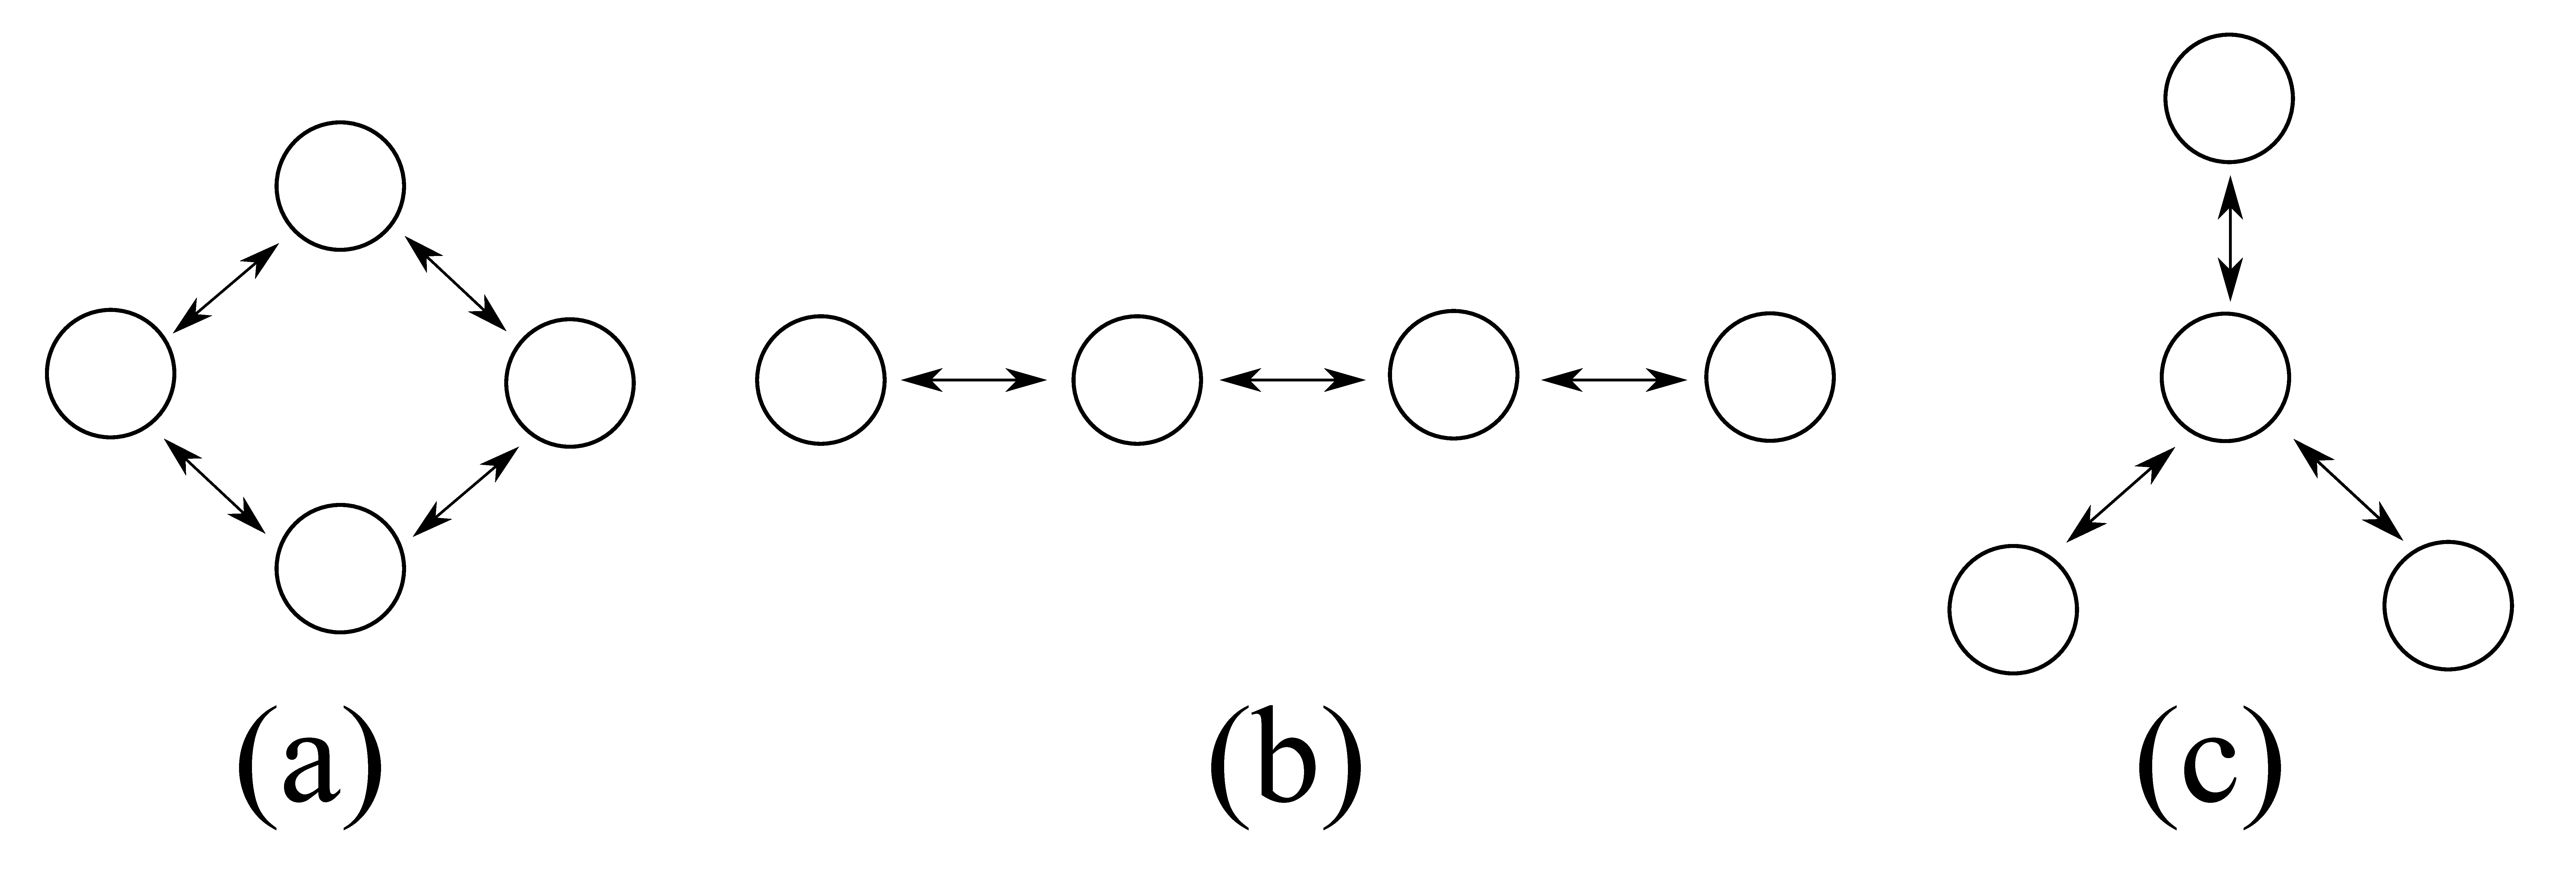
\includegraphics[width=0.42\textwidth]{figures/com_topo}
		\caption{Three types of topologies: (a) ring topology; (b) line topology; (c) star topology}
		\label{fig:com_topo}
		\vspace{-1.3em}
	\end{figure}
	
	%\section{Distributed Bayesian Filter via Latest-In-and-Full-Out Protocol}\label{sec:LIFO-dbf}
	
	
	\subsection{Latest-In-and-Full-Out (LIFO) Protocol}\label{subsec:LIFO}
	%This study proposes a Latest-In-and-Full-Out (LIFO) protocol for observation exchange and derives two corresponding distributed Bayesian filtering (DBF) algorithms, shorted as LIFO-DBF. 
	%The data communication in LIFO uses synchronized step as the execution of DBF.
	%In each step, LIFO only allows single-hopping communication within the direct neighborhood, but is able to broadcast observations of each UGV to any other agents after a finite number of steps.
	%The individual PDF is forward predicted and updated in DBF after each LIFO cycle.
	%The theoretical analysis show that LIFO-DBF can ensure the consistency and consensus of distributed estimation while requiring much less communication burden than statistics dissemination-based methods. 
	This study proposes a Latest-In-and-Full-Out (LIFO) protocol for observation exchange.
	Under LIFO, each UGV contains a communication buffer (CB) to store its latest knowledge of observations of all UGVs: 
	\begin{equation*}
		\mathbf{z}^{CB,i}_k=\left[ z^1_{k^i_1},\dots,z^N_{k^i_N}\right]
	\end{equation*}
	where $z^j_{k^i_j}$ represents the observation made by ${j^\text{th}}$ UGV at time $k^i_j$. 
	Note that under LIFO and certain conditions of interaction topologies, $\mathcal{Q}_i=\left\lbrace 1,\dots,N\right\rbrace \setminus \left\lbrace i\right\rbrace$, which will be proved in \Cref{cor1}.
	$z^j_{k^i_j}$ is stored in the CB of ${i^\text{th}}$ UGV, where $k^i_j$ is the latest observation time of ${j^\text{th}}$ UGV that is available to ${i^\text{th}}$ UGV by time $k$. Due to the communication delay, $k^i_j<k, \forall j\neq i$ and $k^i_i=k$ always holds.
	Let $G[k]\in\bar{G} $ represent the interaction topology at time $k$. 
	The \textbf{LIFO protocol} is stated in \cref{alg:lifo}.
	For the clarity of explanation of DBF in \cref{sec:LIFO-dbf}, we define a \textit{new observation set} $\mathbf{z}^{new,i}_k$ for $i^\text{th}$ UGV to denote the set of observations that the $i^\text{th}$ UGV receives and stores in its CB.% at $k$.
	
	\begin{algorithm}
		\caption{LIFO Protocol}
		\label{alg:lifo}
		\begin{algorithmic}
			\State \textbf{(1)} Initialization:
			The CB of $i^\text{th}$ UGV is initialized when $k=0$,
			\begin{equation*}
				%$\begin{array}{c}
				z^j_{k^i_j}=\varnothing,\; k^i_j=0,\;j=1,\dots,N
				%\end{array}$\\
			\end{equation*}
			
			\State \textbf{(2)} At $k^\text{th}\,(k\geq 1)$ step for $i^\text{th}$ UGV:	
			
%			\State The interaction topology is represented by $G[k]\in\bar{G}$.
			\State (2.1) Receiving Step:
			
			The $i^\text{th}$ UGV receives all CBs of its direct neighborhood $\mathcal{N}_i(G[k-1])$.
			The received CBs are totally $|\mathcal{N}_i(G[k-1])|$ groups, each of which corresponds to the $(k-1)^\text{th}$ step CB of a UGV in $\mathcal{N}_i(G[k-1])$. 
			The received CB from $l^\text{th}$  $\left(l\in \mathcal{N}_i(G[k-1])\right)$ UGV is denoted as
			\begin{equation*}
				\mathbf{z}^{CB,l}_{k-1}=\left[ z^1_{(k-1)^l_1},\dots,z^N_{(k-1)^l_N}\right],\; l\in\mathcal{N}_i(G[k-1])
			\end{equation*}
			
			\State (2.2) Observation Step: 
			
			The $i^\text{th}$ UGV updates $z^j_{k^i_j}\,(j=i)$ by its own observation at current step.
			\begin{align*}
			\text{add}\; & z^i_k\; \text{to}\; \mathbf{z}^{new,i}_k,\\
			z^j_{k^i_j}&=z^i_k,\;k^i_j=k,\;\text{if }j=i.
			\end{align*}
%			\begin{equation*}
%				z^j_{k^i_j}=z^i_k,\;k^i_j=k,\;\text{if }j=i.
%			\end{equation*}
			
			
			\State (2.3) Comparison Step:
			
			The $i^\text{th}$ UGV updates other elements of its own CB, i.e., $z^j_{k^i_j}\,(j\neq i)$, by selecting the latest information among all received CBs from $\mathcal{N}_i(G[k-1])$. For all $j\neq i$,
			\begin{align*}
				l_\text{latest}&=\argmax_{l\in \mathcal{N}_i,\;i}\left\lbrace\left(k-1\right)^i_j,\left(k-1\right)^l_j  \right\rbrace\\
				\text{If}\; l_\text{latest} &> (k-1)^i_j,\;\text{add $z^i_{(k-1)^{l_\text{latest}}_j}$ \text{to} $\mathbf{z}^{new,i}_k$.}\\
				z^j_{k^i_j}&=z^j_{\left(k-1\right)^{l_\text{latest}}_j},\; k^i_j=\left(k-1\right)^{l_\text{latest}}_j.
			\end{align*}
			
			\State (2.4) Sending Step:
			
			The $i^\text{th}$ UGV broadcasts its updated CB to all of its neighbors defined in $\mathcal{N}_i(G[k])$.
			%\bottomrule
			%\end{tabular}
			
			\State \textbf{(3)} $k\leftarrow k+1$ until stop %$\hfill\blacksquare$
		\end{algorithmic}
	\end{algorithm}
	
	\medskip
	\begin{rem}
		Compared to statistics dissemination, LIFO is generally more communication-efficient for distributed filtering. 
		To be specific, consider a $D\times D$ grid environment with a network of $N$ UGVs, the transmitted data of LIFO between each pair of UGVs are only the CB of each UGV and the corresponding UGV positions where observations were made, the length of which is $O(N)$. 
		On the contrary, the length of transmitted data for a statistics dissemination approach that transmits unparameterized posterior distributions or likelihood functions is $O(D^2)$, which is in the order of environmental size. 
		Since $D$ is generally much larger than $N$ in applications such as target localization, LIFO requires much less communication resources.
	\end{rem}
	
	\medskip
%	\todohere{change the figure to be a switching topology. change the contents here accordingly}
	\cref{fig:LIFO} illustrates the LIFO cycles of a network of 3 UGVs with switching line topologies.
	There are two types of topologies: under the first one only UGV $1$ and UGV $2$ can directly communicate and under second one only UGV $2$ and UGV $3$ can directly communicate.
	Several facts can be noticed in \cref{fig:LIFO}: 
	(1) the two topologies are jointly connected within each time intervals $\left[0,3 \right) ,\,\left[3,5 \right) ,\,\left[5,7 \right)$;
	(2) CBs of all UGVs are filled within $5$ steps;
%	, which means under LIFO each UGV has a maximum delay of 2 steps for receiving observations from other UGVs; 
	(3) after being filled, each CB keeps updated every finite time steps, which means each UGV receives new observations of other UGVs with finite delay.
	Extending these facts to a network of $N$ UGVs, we have the following proposition:
	%\medskip
	
	\begin{figure}%[thpb]
		\centering
		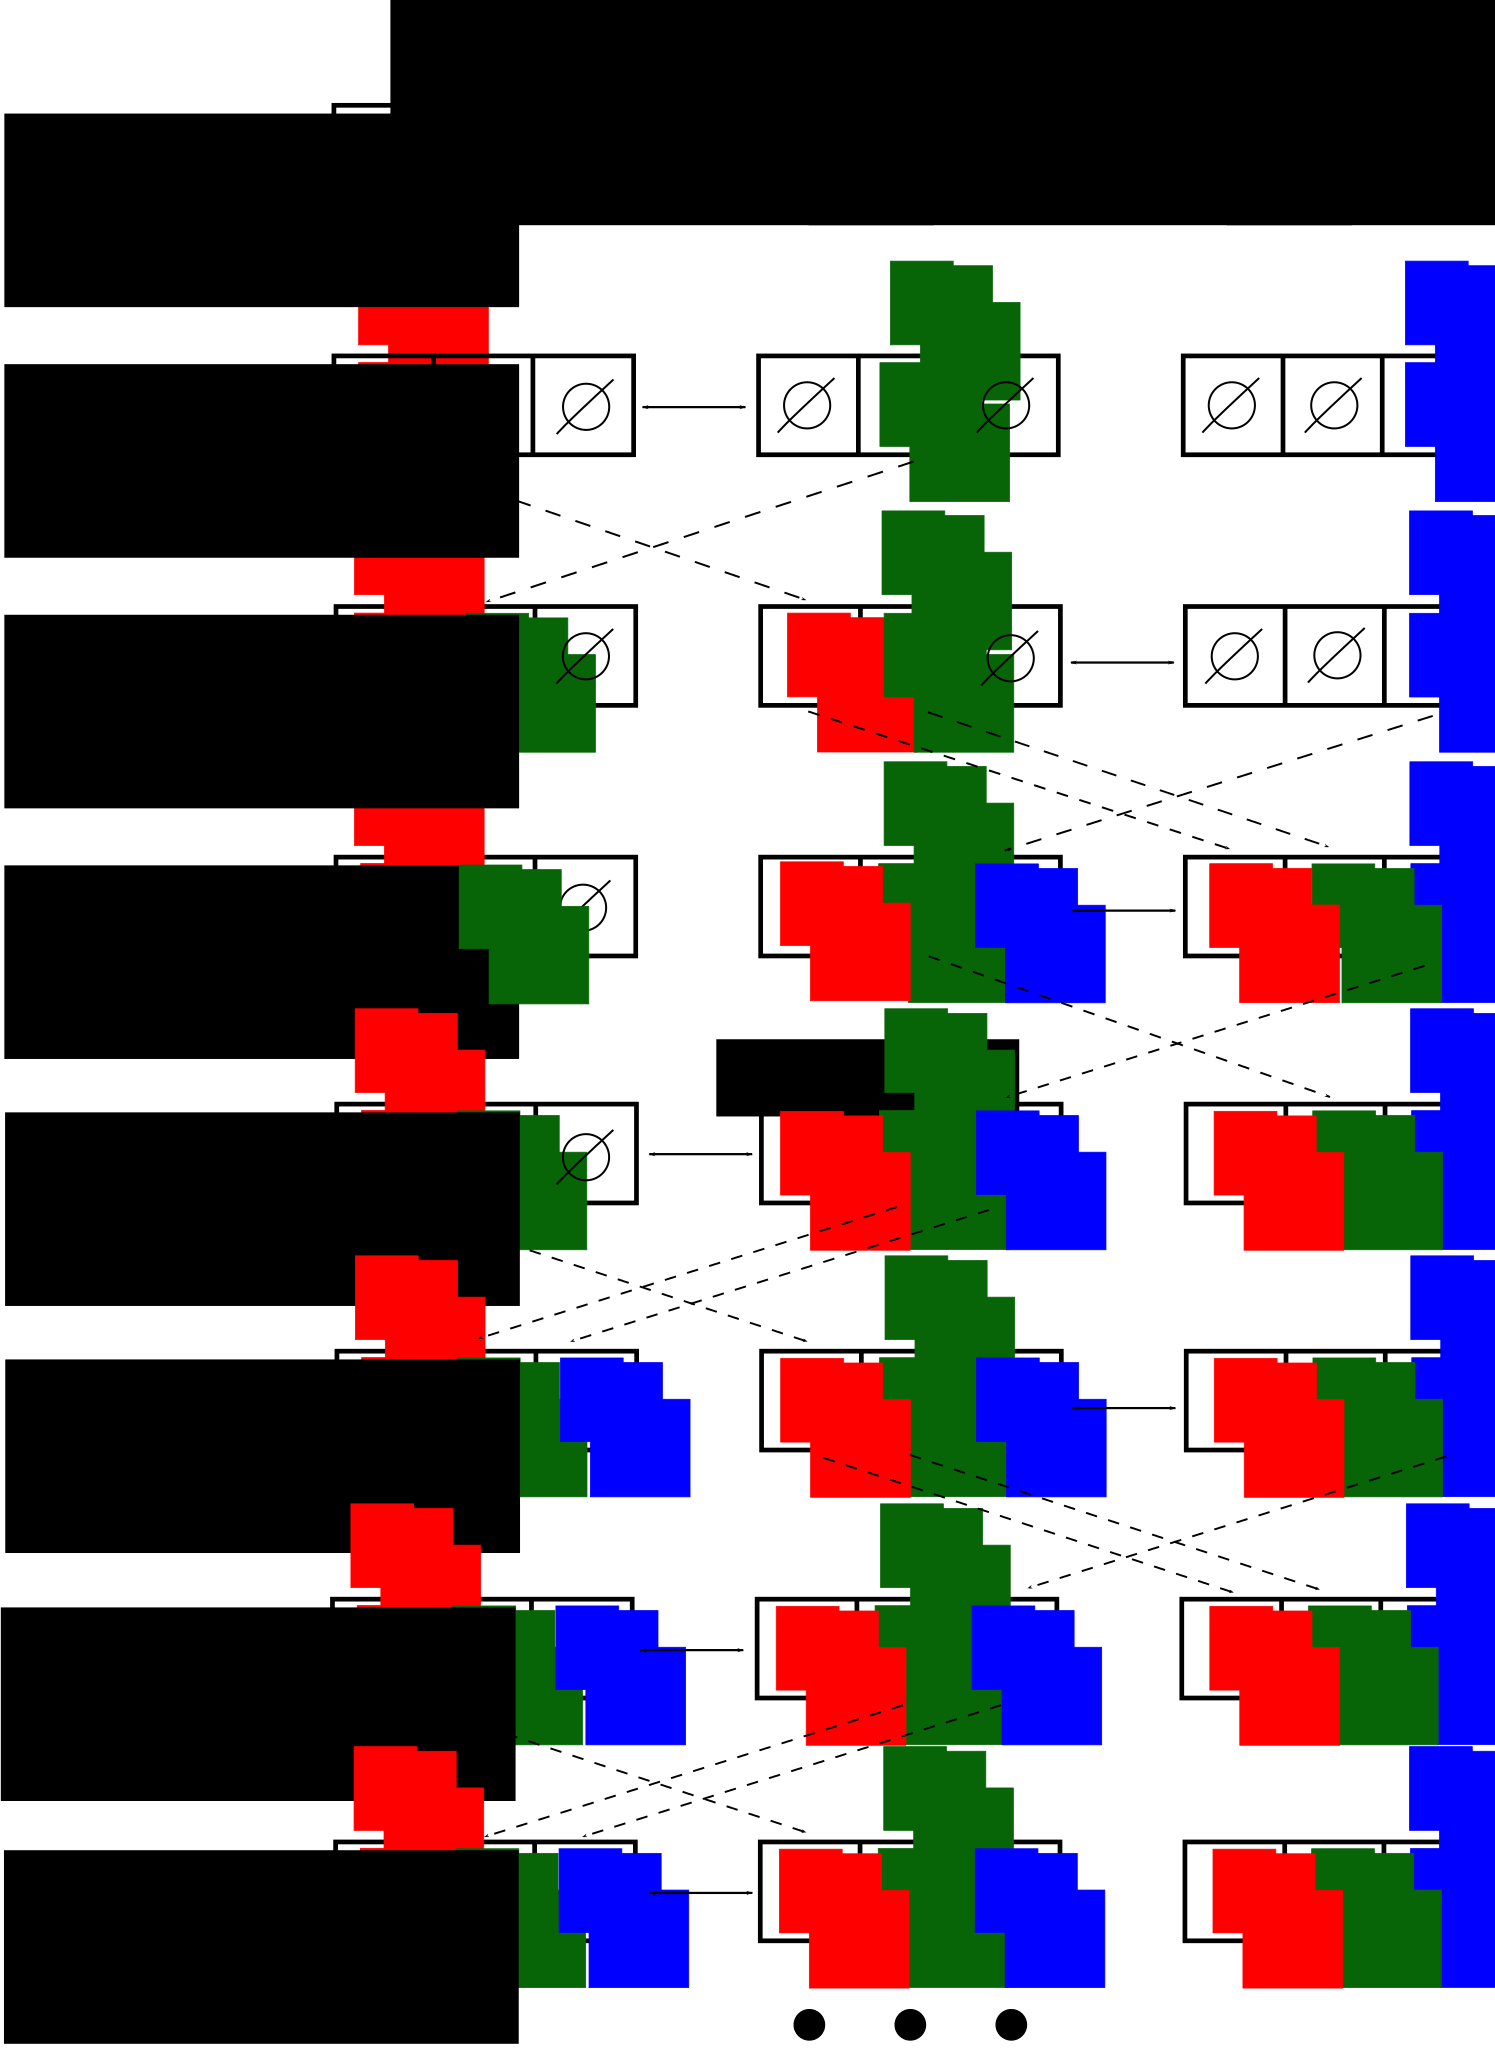
\includegraphics[width=0.42\textwidth]{figures/data_exchange_switch}
		\caption{Example of LIFO with three UGVs using switching line interaction topologies. The double-headed arrow represents a communication link between two UGVs.}
		\label{fig:LIFO}
		\vspace{-1.3em}]
	\end{figure}
	
	\begin{prop}\label{prop1}
		%For a fixed and undirected network of $N$ UGVs, LIFO uses the shortest path(s) between $i^\text{th}$ and $j^\text{th}$ UGV to exchange observation, the length of which is the delay $\tau_{i,j}$ between these two UGVs.
		Consider a network of $N$ UGVs with undirected switching interaction topologies.
%		\todohere{may rephrase the following sentence}
		If the following two conditions are satisfied:
		(1) there exists an infinite sequence of time intervals $\left[k_m,k_{m+1} \right),\,m=1,2,\dots$, starting at $k_1=0$ and are contiguous, nonempty and uniformly bounded;
		(2) the union of graphs across each such interval is jointly connected,
		then arbitrary pair of UGVs can exchange observations under LIFO. In addition, the delay between each pair of UGVs is no greater than \small$(N-1)T_u$\normalsize, where \small$T_u=\sup\limits_{m=1,2,\dots}\left( k_{m+1}-k_m\right) T$ \normalsize is the upper bound of interval lengths.
	\end{prop}
	
	\begin{proof} 
		%Without loss of generality, assume that there is a unique shortest path between $i$ and $j$, denoted by $T^{j,i}_{n^*}=\left(v_1,\dots,v_{n^*}\right)$, with $v_1=j,v_{n^*}=i,v_{m+1}\in\mathcal{N}_{v_m}$. 
		%Then, the distance between $i$ and $j$ is $d(j,i)=n^*-1$. 
		%The following mathematical induction will prove \Cref{prop1}.
		%
		%Step (1): When $d(j,i)=1$, $j\in\mathcal{N}_i$ and $j$ can directly send $z^j_k$ to $i$. Then $z^j_k$ is stored in $i^\text{th}$ CB at time $k+1$, i.e. $\tau_{i,j}=1$. 
		%\Cref{prop1} holds for $d(j,i)=1,\,\forall i,j\in\left\lbrace 1,\dots,N\right\rbrace $.
		%
		%Step (2): Suppose that \Cref{prop1} holds for $d(j,i)=s,\,s\geq 2,\,\forall i,j\in\left\lbrace 1,\dots,N\right\rbrace$. 
		%Then for $d(j,i)=s+1$, i.e., $n^*=s+2$, by the Bellman's principle of optimality, the path $T^{j,l}_{n^*-1}=\left(v_1,\dots,v_{n^*-1}\right)$ is a shortest path between $j$ and $l$, where $v_{n^*-1}=l$ and $i\in \mathcal{N}_l$. 
		%The assumption that \Cref{prop1} holds for $d(j,i)=s$ implies that $z^j_k$ is received and stored in $l^\text{th}$ UGV's CB at time $k+s$. 
		%Since $i\in\mathcal{N}_l$, $i^\text{th}$ UGV receives $z^j_k$ at $k+s+1$. 
		%For any other path $T^{j,i}_{n}=\left(v_1,\dots,v_{n}\right)$ with $n>n^*$, $z^j_k$ cannot be received by $i$ earlier than $k+s+1$. 
		%Therefore $\tau_{i,j}=s+1$. 
		%This proves the \Cref{prop1} for $d(j,i)=s+1$.
		Consider the transmission between two arbitrary UGVs, $i$ and $j$.
%		 $i^\text{th}$ and $j^\text{th}$ UGV.
		%Without loss of generality, we focus on the transmission of $z^i_0$, the observation at time $0$ by $i^\text{th}$ UGV.
		Since the union of graphs across time interval $\left[k_1,k_2 \right)$ is jointly connected, $i^\text{th}$ UGV can directly communicate with at least one another UGV at a time instance, i.e., $\exists l_1\in V,\,t_1\in \left[k_1,k_2 \right)$ such that $i\in\mathcal{N}_{l_1}(G[t_1])$.
		This implies that observation $z^i_{t_1}$ is received and stored in the CB of $l_1^\text{th}$ UGV at $t_1+1$ under LIFO.
		Therefore, at least one UGV other than $i^\text{th}$ UGV has received and received observation from $i^\text{th}$ UGV by $k_2$.
		If $l_1=j$, then we have proved the exchange of observations between $i$ and $j$.
		If $l_1\neq j$, we consider time interval $\left[k_2,k_3 \right)$.
		By using similar derivation as before, it is easy to understand that $\exists l_2\in V,\,t_2\in \left[k_2,k_3 \right)$ such that $i\in\mathcal{N}_{l_2}(G[t_2])$ or $l_1\in\mathcal{N}_{l_2}(G[t_2])$.
		For the former case, $z^i_{t_2}$ is received and stored in the CB of $l_2^\text{th}$ UGV at $t_2+1$ under LIFO;
		for the latter case, $z^i_{t_1}$ is received by $l_2^\text{th}$ UGV at $t_2+1$ but may not be stored in its CB.
		This happens if $l_2^\text{th}$ UGV has received a newer observation $z^i_{t^\prime_2},\,t_1<t^\prime_2<t_2$, from UGVs other than $l_1$.
		In both cases, at least two UGVs have received and stored an observation from $i^\text{th}$ UGV by $k_3$.
		Using similar derivation, it can be shown that all $N-1$ UGVs, except $i^\text{th}$ UGV, will receive and store an observation from $i$ no later by $k_{N}$.
		Therefore, the transmission delay between an arbitrary pair of UGVs is no greater than \small$(N-1)T_u$\normalsize.
	\end{proof}
	%\vspace{\baselineskip}
	\medskip
	\begin{cor}\label{cor1}
		With the same network condition in \Cref{prop1}, all elements in $\mathbf{z}^{CB,i}_k$ under LIFO become filled within finite time, i.e., $\mathcal{Q}_i = \left\lbrace1,\dots,N \right\rbrace \setminus \left\lbrace i\right\rbrace $.	
		Additionally, each element keeps updated every finite period of time.
	\end{cor}
	\begin{proof}
		%In a network of $N$ UGVs, the maximal length of shortest paths is no greater than $N-1$. 
		According to \Cref{prop1}, the transmission delay between an arbitrary pair of UGVs is no greater than \small$(N-1)T_u$\normalsize.
		Therefore, CBs of all UGVs becomes filled when \small$k\geq (N-1)T_u$\normalsize.
		In addition, each element in CBs gets updated every finite period of time no greater than \small$(N-1)T_u$\normalsize.
		%$\tau_{i,j}\leq N-1$ and thus all elements of $\mathbf{z}^{CB,i}_k$ become filled when $k\geq N$.
	\end{proof}
	
	\medskip
	
	%\begin{rem}
	%	The \cref{prop1} provides an upper bound of the transmission delay between arbitrary pair of UGVs.
	%	One example of such delay can be found in line topology as shown in \cref{fig:com_topo}.
	%	\todohere{needs to write more details.}
	%%	Suppose three types of graphs that consists Consider the tranmission
	%\end{rem}
	%\medskip
	%\begin{cor}\label{cor2}
	%For the same network condition in \Cref{prop1}, all elements in $\mathbf{z}^{CB,i}_k$ are filled, the updating of each element is non-intermittent. 	
	%\end{cor}
	%\begin{proof}
	%For a network with fixed topology, shortest path(s) between any pair of nodes are fixed. 
	%Therefore, based on \Cref{prop1}, $\tau_{i,j}$ is constant and the updating of each element in $\mathbf{z}^{CB,i}_k$ is non-intermittent.
	%\end{proof}
	%\medskip
	
	\section{Distributed Bayesian Filter via Latest-In-and-Full-Out Protocol}\label{sec:LIFO-dbf}
	
	
	\subsection{Probabilistic Model of Binary Sensor}
	%In this paper, distributed Bayesian filter is used to estimate the true target position by a network of binary sensors.
	In this study, each UGV is equipped with a binary sensor, which only gives two types of observation: $1$ if the target is detected, and $0$ if no target is detected. 
	The observation of $i^\text{th}$ sensor at $k^\text{th}$ time step is denoted as $z^i_k$.
	% and subjects to Bernoulli distribution $B(1,p_{i,k})$.
	The likelihood function that the target is detected is
	%The following likelihood function gives the probability for $i^\text{th}$ sensor to obtain $z^i_k$:
	%\small\begin{equation}\label{eqn:bin_sensor}
	%	P(z^i_k|x^T_k;x^R_k)=p^{z^i_k}_{i,k}(1-p_{i,k})^{1-z^i_k},
	%\end{equation}\normalsize
	%where $p_{i,k}=P(z^i_k=1|x^T_k;x^R_k)$; $x^T_k$ and $x^R_k$ denote the target and UGV position at $k$, respectively.
	\small\begin{equation}\label{eqn:bin_sensor1}
	P(z^i_k=1|x^T;x^{R,i})\in \left[0,1\right],\; x^T\in S,
	\end{equation}\normalsize
	where $x^T$ denotes the target position; $x^{R,i}$ is the position of $i^\text{th}$ UGV.
	%; $X^T$ represents the set of all possible target positions.
	Correspondingly, the likelihood function that no target is detected is
	\small\begin{equation}\label{eqn:bin_sensor0}
	P(z^i_k=0|x^T;x^{R,i})=1-P(z^i_k=1|x^T;x^{R,i}).
	\end{equation}\normalsize
	%\Cref{eqn:bin_sensor} actually defines a binary sensor model parameterized by $x^T_k$ and $x^R_k$.
	
	The combination of \Cref{eqn:bin_sensor1} and \Cref{eqn:bin_sensor0} forms a binary sensor model parameterized by $x^T$ and $x^{R,i}$. 
	For the purpose of simplicity, we will not explicitly write $x^{R,i}$ when no confusion may occur.
	%, with which all observations are generated. 
	The commonly used likelihood functions for binary sensor include Gaussian function \cite{bonnie2012modelling,liu2015model} and step function \cite{djuric2008target}.
	
%	\begin{rem}
%		Given the knowledge of current target and UGV positions, current observation of each UGV is conditionally independent from its own past observations and those of other UGVs.
%	\end{rem}
	
%	\begin{rem} 
%		The proposed LIFO protocol 
%		%to be described in \cref{sec:LIFO-dbf} 
%		is applicable for both homogeneous and heterogeneous binary sensors. 
%		A homogeneous model can simplify the analysis of LIFO-based DBF, while a heterogeneous model is more close to real sensing characteristics.
%		In addition, it also works for other types of sensors, such as laser scanners and cameras.
%	\end{rem}	
	
	\subsection{Distributed Bayesian Filter for Multiple UGVs}\label{subsec:dbf}
	
	The distributed Bayesian filter (DBF) using LIFO protocol is introduced in this section.
	%, which is also stated in \cite{bandyopadhyay2014distributed} and \cite{julian2012distributed}. 
	Each UGV has its individual estimation of posterior density function (PDF) of target position, called \textit{individual PDF}. 
	The individual PDF of $i^\text{th}$ UGV at time $k$ is defined as
	% ,z^{\mathcal{Q}_i}_{1:k})
	\small$P^i_{pdf}(x^T|\mathbf{z}^{new,i}_{1:k})$\normalsize, where $\mathbf{z}^{new,i}_{1:k}$ denotes the collection of new observation set by $i^\text{th}$ UGV from time $1$ to $k$.
	%and by UGVs in $\mathcal{Q}_i$ that have been stored in CB of $i^\text{th}$ UGV by time $k$.
	%from time $1$ through $k$ and $z^{\mathcal{Q}_i}_{1:k}$ means the set of observations by UGVs in $\mathcal{Q}_i$ that are transmitted to $i^\text{th}$ UGV.
	%Note that if the observation by $j^\text{th}(j\in \mathcal{Q}_i)$ UGV at time $k'(k'\leq k)$ is not received by $i^\text{th}$ UGV, the corresponding element $z^j_{k'}$ in $z^{\mathcal{Q}_i}_{1:k}$ is empty and thus not utilized for computing $i^\text{th}$ individual PDF.
	The individual PDF is initialized as \small$P^i_{pdf}(x^T|\mathbf{z}^{new,i}_0)=P(x^T)$\normalsize,
	%$P^i_{pdf}(x^T_0|z^i_0,z^{\mathcal{Q}_i}_0)=P(x^T_0)$, 
	given all available prior information including past experience and environmental knowledge. Under the framework of DBF, the individual PDF is recursively estimated using Bayes' formula, based on observations of $i^\text{th}$ UGV and that of UGVs in $\mathcal{Q}_i$.
	
%	\subsubsection{Prediction}
%	%The $i^\text{th}$ individual PDF at time $k-1$ is known, denoted as $P^i_{pdf}(x^T_{k-1}|z^i_{1:k-1},z^{\mathcal{Q}_i}_{1:k-1})$. 
%	%At time $k$, the prior individual PDF $P^i_{pdf}(x^T_{k-1}|z^i_{1:k-1},z^{\mathcal{Q}_i}_{1:k-1})$ is first predicted forward by using the Chapman-Kolmogorov equation:
%	At time $k$, the prior individual PDF $P^i_{pdf}(x^T_{k-1}|\mathbf{z}^{new,i}_{1:k-1})$ is first predicted forward by using the Chapman-Kolmogorov equation:
%	%\small\begin{align}\label{eqn:bayes_pred}
%	%&P^i_{pdf}(x^T_k|z^i_{1:k-1},z^{\mathcal{Q}_i}_{1:k-1})\notag\\
%	%&=\int P(x^T_k|x^T_{k-1})P^i_{pdf}(x^T_{k-1}|z^i_{1:k-1},z^{\mathcal{Q}_i}_{1:k-1})dx^T_{k-1}
%	%\end{align}\normalsize
%	\small\begin{equation}\label{eqn:bayes_pred}
%		P^i_{pdf}(x^T_k|\mathbf{z}^{new,i}_{1:k-1})
%		=\int P(x^T_k|x^T_{k-1})P^i_{pdf}(x^T_{k-1}|\mathbf{z}^{new,i}_{1:k-1})dx^T_{k-1}
%	\end{equation}\normalsize
%	where $P(x^T_k|x^T_{k-1})$ is a Markov motion model of the target, independent of UGV states. 
%	This model describes the state transition probability of the target from a prior state $x^T_{k-1}$ to posterior state $x^T_k$. 
%	Note that the target is static in many search applications, such as the indoor search for stationary objects \cite{kulich2014single}. 
%	For a static target, its Markov motion model is simplified to be
%	\small\begin{equation*}
%		P(x^T_k|x^T_{k-1})=\begin{cases}
%			1 & \text{if}\; x^T_k=x^T_{k-1}\\
%			0 & \text{if}\; x^T_k\neq x^T_{k-1}
%		\end{cases}.
%	\end{equation*}\normalsize
%	%and \Cref{eqn:bayes_pred} can be reduced to $P^i_{pdf}(x^T_{k}|z^i_{1:k-1},z^{\mathcal{Q}_i}_{1:k-1})=P^i_{pdf}(x^T_{k-1}|z^i_{1:k-1},z^{\mathcal{Q}_i}_{1:k-1})$.
%	This work focuses on the localization of static target.
%	Therefore, we remove the subscript of $x^T_k$ for the rest of the paper.
	
%	\subsubsection{Updating}
	To be specific, at time $k$, the $i^\text{th}$ individual PDF is updated using the set of newly received observations $\mathbf{z}^{new,i}_k$:
	%\small\begin{align}\label{eqn:bayes_upd}
	%&P^i_{pdf}(x^T_k|z^i_{1:k},z^{\mathcal{Q}_i}_{1:k})\notag\\
	%&=K_iP^i_{pdf}(x^T_k|z^i_{1:k-1},z^{\mathcal{Q}_i}_{1:k-1})P(z^i_k|x^T_k)\prod\limits_{j\in\mathcal{Q}_i}P(z^j_k|x^T_k)
	%\end{align}\normalsize
	%\small\begin{equation}\label{eqn:bayes_upd}
	%P^i_{pdf}(x^T_k|\mathbf{z}^i_{1:k})
	%=K_iP^i_{pdf}(x^T_k|\mathbf{z}^i_{1:k-1})P(z^i_k|x^T_k)\prod\limits_{j\in\mathcal{Q}_i}P(z^j_k|x^T_k)
	%\end{equation}\normalsize
	%\small\begin{equation}\label{eqn:bayes_upd}
	%P^i_{pdf}(x^T_k|\mathbf{z}^{new,i}_{1:k})
	%=K_iP^i_{pdf}(x^T_k|\mathbf{z}^{new,i}_{1:k-1})P(\mathbf{z}^{new,i}_k|x^T_k)
	%\end{equation}\normalsize
	\small\begin{align}\label{eqn:bayes_upd}
		P^i_{pdf}(x^T|\mathbf{z}^{new,i}_{1:k})
		&=K_iP^i_{pdf}(x^T|\mathbf{z}^{new,i}_{1:k-1})P(\mathbf{z}^{new,i}_k|x^T)\notag\\
		&=K_iP^i_{pdf}(x^T|\mathbf{z}^{new,i}_{1:k-1})\prod\limits_{z^j_{k^i_j}\in \mathbf{z}^{new,i}_k}P(z^j_{k^i_j}|x^T)dx^T.
	\end{align}\normalsize
	where $K_i$ is a normalization factor, given by
	%\small\begin{align*}
	%K_i=1/\int P^i_{pdf}(x^T_k|z^i_{1:k-1},z^{\mathcal{Q}_i}_{1:k-1})P(z^i_k|x^T_k)\prod\limits_{j\in\mathcal{Q}_i}P(z^j_k|x^T_k)dx^T_k
	%\end{align*}\normalsize
	%\small\begin{align*}
	%K_i=1/\int P^i_{pdf}(x^T_k|\mathbf{z}^i_{1:k-1})P(z^i_k|x^T_k)\prod\limits_{j\in\mathcal{Q}_i}P(z^j_k|x^T_k)dx^T_k
	%\end{align*}\normalsize
	\small\begin{align*}
		%K_i=1/\int P^i_{pdf}(x^T_k|\mathbf{z}^{new,i}_{1:k-1})P(\mathbf{z}^{new,i}_k|x^T_k)dx^T_k
		K_i=1/\int P^i_{pdf}(x^T|\mathbf{z}^{new,i}_{1:k-1})\prod\limits_{z^j_{k^i_j}\in \mathbf{z}^{new,i}_k}P(z^j_{k^i_j}|x^T)dx^T,
	\end{align*}\normalsize
	and $P^i_{pdf}(x^T|\mathbf{z}^{new,i}_{1:k})$ is called posterior individual PDF; $P(z^j_{k^i_j}|x^T)$ is the likelihood function of observation $z^j_{k^i_j}$, described in \Cref{eqn:bin_sensor1} and \Cref{eqn:bin_sensor0}.
	Note that the factorization of $P(\mathbf{z}^{new,i}_k|x^T)$ in \Cref{eqn:bayes_upd} results from the conditional independence of observations by different UGVs given the position of the target.
	
	%Utilizing the conditional independence property of observations, $P(\mathbf{z}^{new,i}_k|x^T)$ can be further factorized:
	%\small\begin{equation}\label{eqn:LIFO-dbf-sta-tar}
	%P^i_{pdf}(x^T|\mathbf{z}^{i}_{1:k})=K_iP^i_{pdf}(x^T|\mathbf{z}^{i}_{1:k-1})\prod\limits_{j=1}^{N}P(z^j_{k^i_j}|x^T)
	%\end{equation}\normalsize
	
	
	
	
	%\todohere{merge this section with previous one}
	%\subsection{Algorithm of LIFO-DBF for Static Target}\label{subsec:LIFO-dbf-sta-tar} 
	
	%This section derives the LIFO-DBF algorithm for localizing a static target. 
	%Each UGV stores last-step individual PDF, i.e., $P^i_{pdf}(x^T|\mathbf{z}^{i}_{1:k-1})$. 
	%According to \Cref{cor2}, $\mathbf{z}^i_k=\mathbf{z}^{CB,i}_k$ and $\mathbf{z}^{i}_{1:k}=\mathbf{z}^{CB,i}_{1:k}=\left[ z^1_{1:k^i_1},\dots,z^N_{1:k^i_N}\right]$.
	%The assumption of static target can simplify the Bayesian filter as the prediction step becomes unnecessary. 
	%Therefore, the $i^\text{th}$ individual PDF is only updated by 
	%\small\begin{align}\label{eqn:LIFO-dbf-sta-tar}
	%P^i_{pdf}(x^T|\mathbf{z}^{i}_{1:k})&=K_iP^i_{pdf}(x^T_k|\mathbf{z}^i_{1:k-1})P(\mathbf{z}^i_k|x^T_k)\notag\\
	%&=K_iP^i_{pdf}(x^T|\mathbf{z}^{i}_{1:k-1})\prod\limits_{j=1}^{N}P(z^j_{k^i_j}|x^T)
	%\end{align}\normalsize
	
	%\small\begin{equation}\label{eqn:LIFO-dbf-sta-tar}
	%P^i_{pdf}(x^T|\mathbf{z}^{i}_{1:k})=K_iP^i_{pdf}(x^T|\mathbf{z}^{i}_{1:k-1})\prod\limits_{j=1}^{N}P(z^j_{k^i_j}|x^T)
	%\end{equation}\normalsize
	%where
	%\small\begin{equation*}
	%K_i=1/\int P^i_{pdf}(x^T|\mathbf{z}^{i}_{1:k-1})\prod\limits_{j=1}^{N}P(z^j_{k^i_j}|x^T)dx^T
	%\end{equation*}\normalsize
	
	%\subsection{Algorithm of LIFO-DBF for Moving Target}\label{subsec:LIFO-dbf-mov-tar}
	%This section derives the LIFO-DBF for localizing a moving target. 
	%Instead of storing last-step PDF, at time $k$ each UGV maintains an individual PDF of time $(k-N)$ and a collection of historical observations, called the \textit{record set}, from time $(k-N+1)$ to $k$. 
	%The $i^\text{th}$ individual PDF is then alternatively predicted and updated by using aforementioned Bayesian filter (\Cref{eqn:bayes_pred} and \Cref{eqn:bayes_upd}) from $(k-N)$ to $k$.
	%\cref{fig:LIFO-DBF} illustrates the LIFO-DBF procedure for the $1^\text{st}$ UGV as an example.
	%With a line topology, the record set of $1^\text{st}$ UGV is shown as a triangle.
	%% shape formed by squares that contain observations from $(k-N+1)$ to $k$.
	%
	%Let $\Omega^i_{\xi}\,\left(\xi=1,\dots,N\right) $ denote the index set of UGVs whose observation at time $(k-N+\xi)$ is stored in $i^\text{th}$ UGV's record set. 
	%The \textbf{LIFO-DBF algorithm} for moving target is then stated in \cref{alg:lifo-dbf}.
	%
	%\begin{figure}%[thpb]
	%	\centering
	%	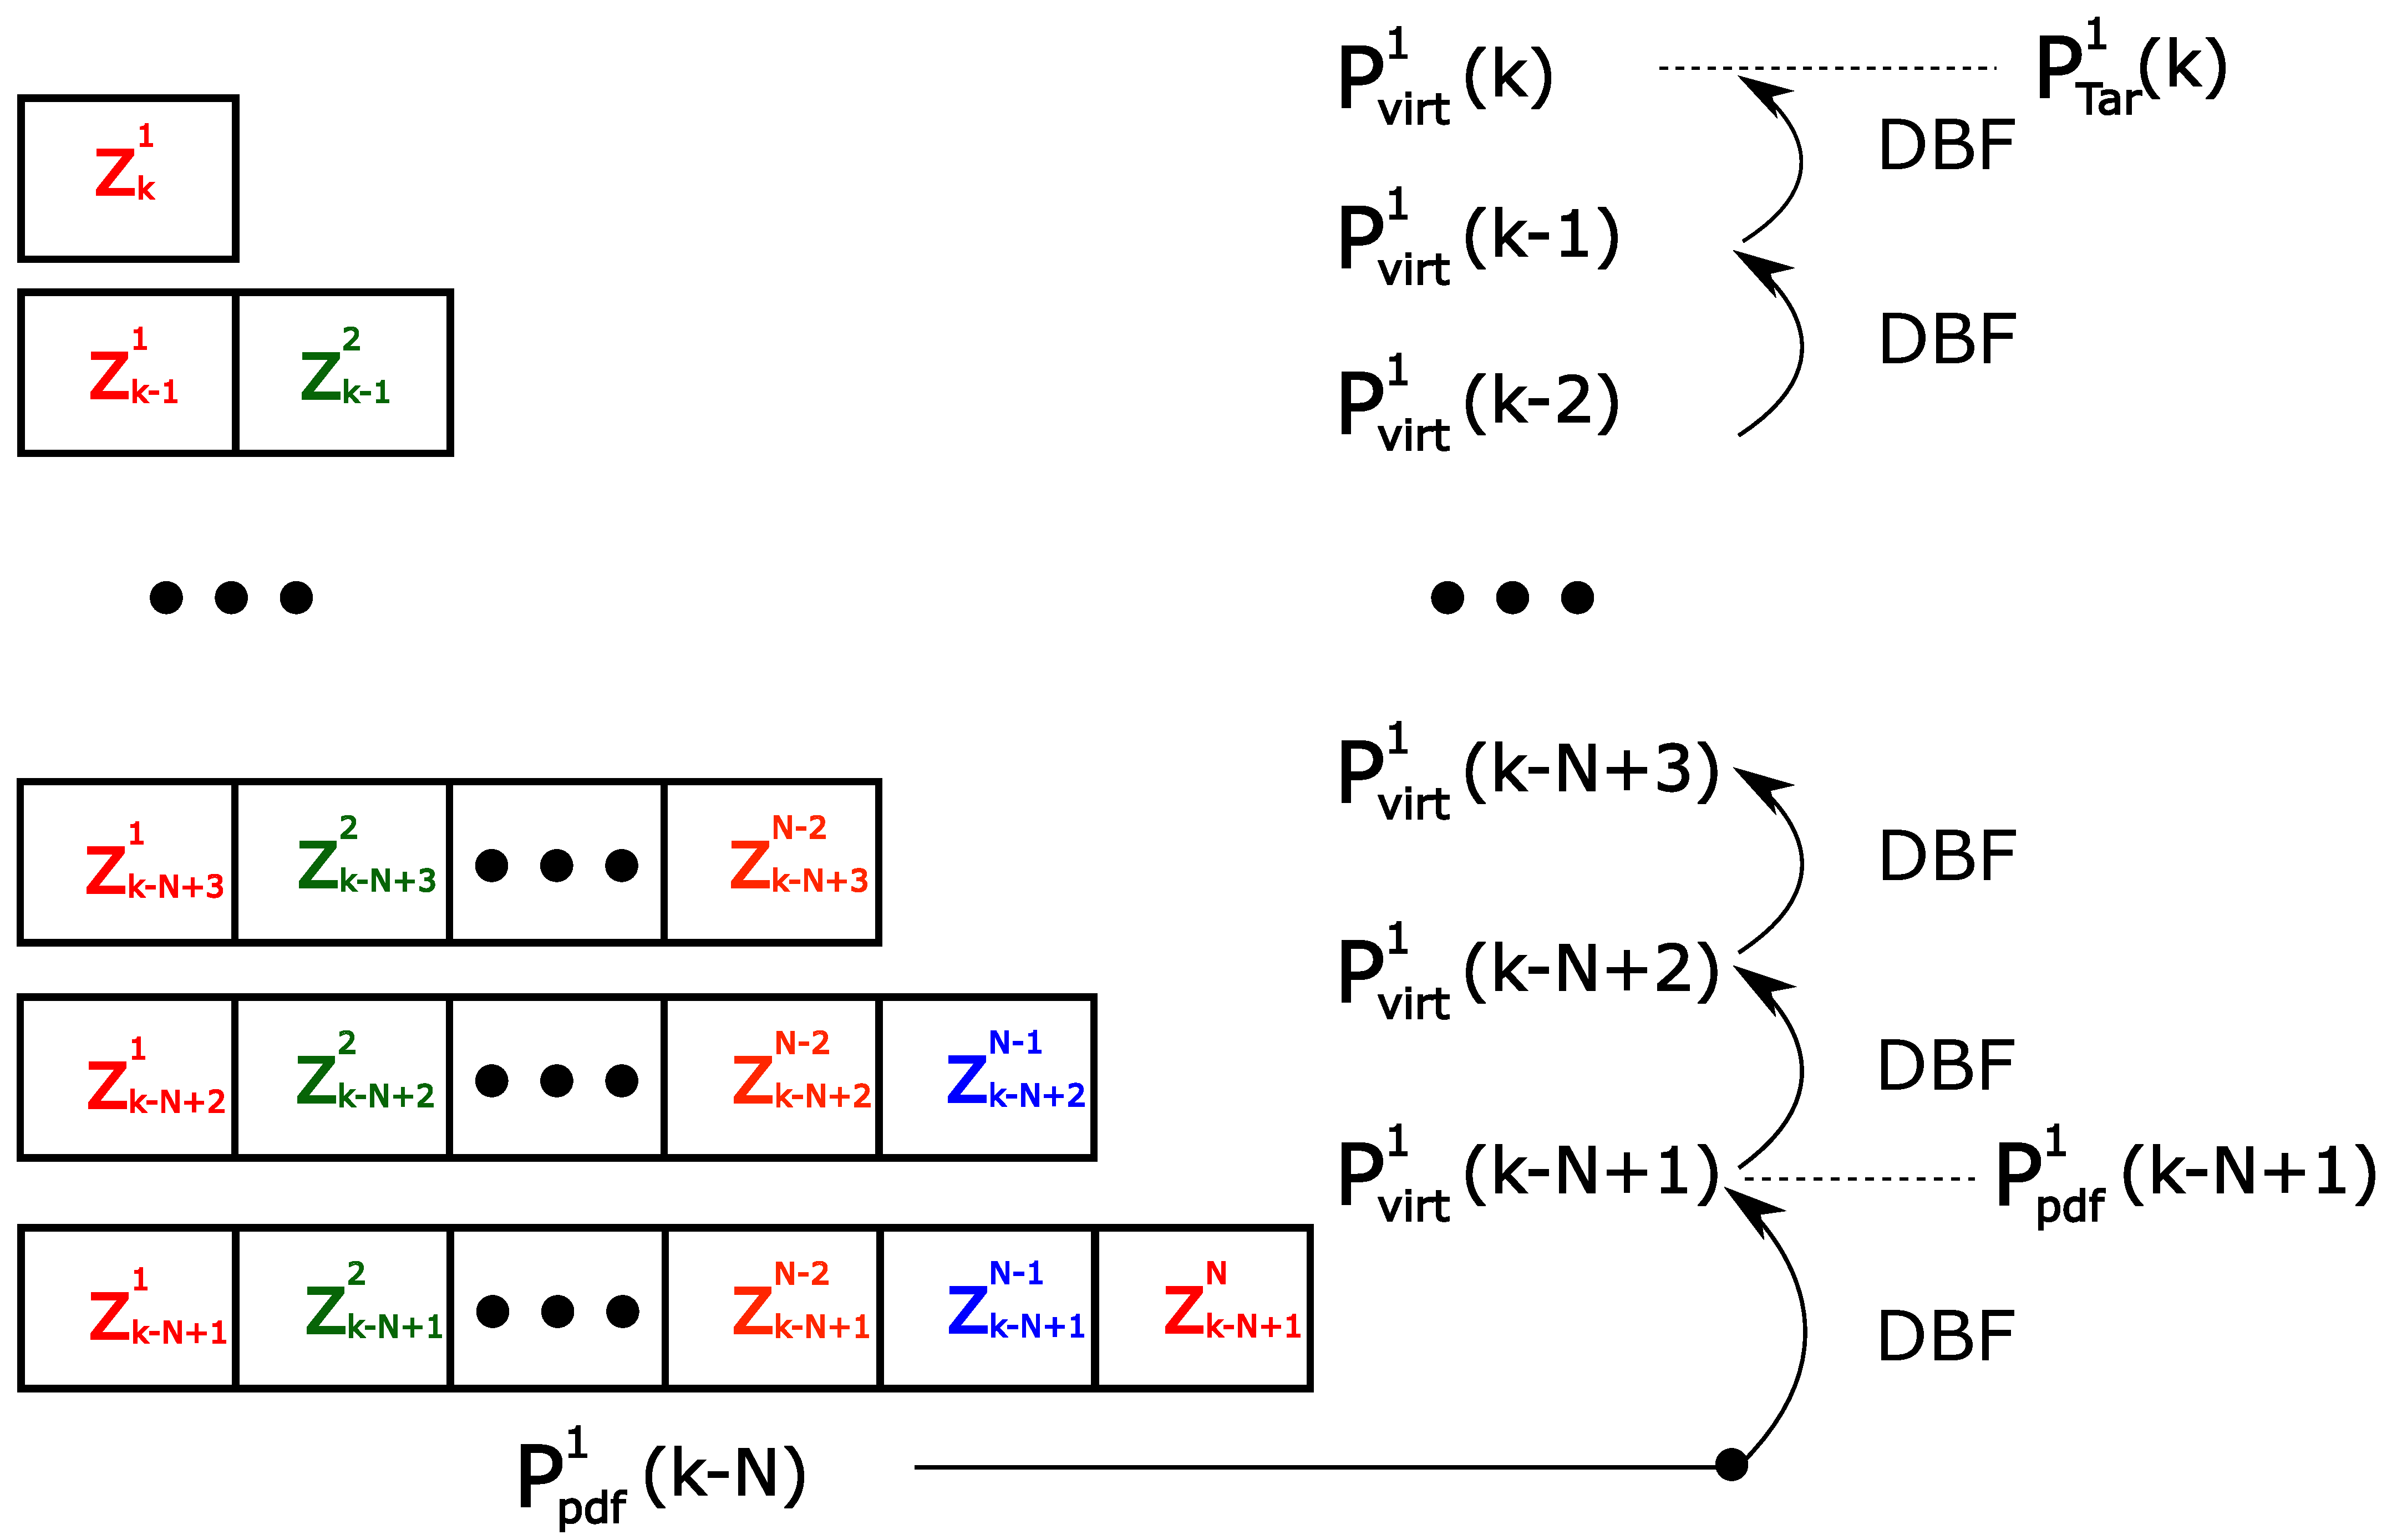
\includegraphics[width=0.47\textwidth]{figures/DBF_demo}
	%	\caption{Example of LIFO-DBF for $1^\text{st}$ UGV at time $k$. 	 
	%		Networked UGVs take a line topology, shown in the top. 
	%		The stored individual PDF is $ P^1_{pdf}(k-N)$.
	%		The UGV first calculates $ P^1_{virt}(k-N+1)$ using DBF and stores it as $ P^1_{pdf}(k-N+1)$. 
	%		Repeating DBF until obtaining $ P^1_{pdf}(k)$, which is then used as the target PDF estimation of $1^\text{st}$ UGV at time $k$.
	%		In this example, $\Omega^1_{\xi}=\left\lbrace 1,2,\dots,N+1-\xi\right\rbrace $, $\xi=1,\dots,N$.}
	%	\label{fig:LIFO-DBF}
	%\end{figure}
	%
	%\begin{rem}
	%	For the static target, each UGV only needs current step CB to update individual PDFs. 
	%	Therefore, besides storing individual PDFs, only current-step CB is stored in UGV memory and all historical CBs can be discarded, which means that the size of occupied memory is $O(N)$. 
	%	On the contrary, for the moving target, each UGV needs to store a triangular matrix of historical observation 
	%%	(except current step CB) 
	%	with size of $O(N^2)$ and an individual PDF with size $O(M^2)$, which means that the size of occupied memory in each UGV is $O(M^2+N^2)$.
	%	\todohere{notation M collides with that of adjacency matrix.}
	%\end{rem}
	
	\subsection{Proof of Consistency}\label{sec:consist_proof}
	%This section proves consistency and consensus of LIFO-DBF. 
	%Only proofs for localizing static target are presented, including static UGVs and moving UGVs.
	%The proof of LIFO-DBF for moving target is similar to that of static target by considering the dynamic model of the target, but with more complicated algebraic manipulation. 
	
	%Considering $S$ is finite and $x^{T^*}$ is the true location of target, define an \textit{equivalent-location} set $X^T_{eq}\subseteq S$ such that 
	%\small\begin{equation*}
	%X^T_{eq}=\left\lbrace x^T\in S\arrowvert P(z_k|x^{T})=P(z_k|x^{T^*}),\; \forall z_k\in \left\lbrace 0,1\right\rbrace\right\rbrace ,
	%\end{equation*}\normalsize
	%i.e., $x^T\in X^T_{eq}$ gives the same observation likelihood as $x^{T^*}$ for given UGV positions.
	%%for any two parameters in $X^T_{eq}$, the sensor model with one of these two parameters generates equivalent probability value for the same observation $z_k$
	%Since $S$ is finite, $X^T_{eq}$ is also finite. 
	%%Let $X^T_{eq,1},\dots,X^T_{eq,u}$ denote all equi-parameter sets that partition $X^T$ such that following properties hold:
	%%\begin{enumerate}
	%%	\item $\bigcup^u_{i=1} X^T_{eq,i}= X^T$
	%%	\item $X^T_{eq,i}\cap X^T_{eq,j}=\emptyset,\;i,j\in \left\lbrace 1,\dots,u\right\rbrace ,i\neq j.$
	%%\end{enumerate}
	%%Without loss of generality, assume $x^{T^*}\in X^T_{eq,1}$, where $x^{T^*}$ denotes the actual position of the target. 
	%
	%%\todohere{double check if the following examples for equi-parameter set are accurate}
	%
	%%\begin{rem}
	%%	the equivalent-location set depends on the property of the sensor. 
	%%	For example, for a laser scanner with high-fidelity sensing capability, each equivalent-location set contains only a small number of target positions.
	%	The reason to introduce equivalent-location set is that ghost target might exist in some special UGV arrangement and sensor types.
	%	For example, for undirected binary sensors that are linearly arranged, a ghost target can exist at the mirror position of the true target.
	%	When sensors are overlapped at a single point, ghost targets can exist on a circle that contains the true target.
	%	In theory, DBF cannot rule out ghost targets in such cases and prior knowledge is needed for further clarification.
	%%	Therefore, this study only proves the convergence to the equivalent-location set rather to the true location.
	%	However, by using high-fidelity sensors, such as cameras and laser scanners, and multiple observations from different UGV placements, equi-location set can be reduced to only contain true location of target.
	
	%\end{rem}
	
	%\begin{algorithm}
	%	\caption{LIFO-DBF Algorithm}\label{alg:lifo-dbf}
	%	\begin{algorithmic}
	%		\State For $i^\text{th}$ UGV at $k^\text{th}$ step:
	%		\State After updating CB by \cref{alg:lifo},	
	%		\State \textbf{(1)} The stored individual PDF for time $(k-N)$ is:
	%		\small\begin{equation*}
	%		P^i_{pdf}(x^T_{k-N}|z^1_{1:k-N},\dots,z^N_{1:k-N})
	%		\end{equation*}\normalsize		
	%		\State\textbf{(2)} Initialize a virtual PDF by assigning the individual PDF to it:
	%		\small\begin{equation*}
	%		P^i_{virt}(x^T_{k-N})=P^i_{pdf}(x^T_{k-N}|z^1_{1:k-N},\dots,z^N_{1:k-N})
	%		\end{equation*}\normalsize		
	%		\State\textbf{(3)} From $\xi=1$ to $N$, repeat two steps of Bayesian filtering:
	%		%	\begin{enumerate}
	%		%		\item 
	%		
	%		\State(3.1) Prediction 
	%		\small\begin{align*}
	%		&P_{virt}^{pre}(x^T_{k-N+\xi})\\=&\int P(x^T_{k-N+\xi}|x^T_{k-N+\xi-1})P^i_{virt}(x^T_{k-N+\xi-1})dx^T_{k-N+\xi-1}
	%		\end{align*} \normalsize
	%		
	%		%		\item 
	%		\State(3.2) Updating
	%		\small\begin{gather*}
	%		P^i_{virt}(x^T_{k-N+\xi})=K_\xi P_{virt}^{pre}(x^T_{k-N+\xi})\prod\limits_{j\in\Omega^i_{\xi}}P(z^j_{k-N+\xi}|x^T_{k-N+\xi})\\
	%		K_\xi=1/\int P_{virt}^{pre}(x^T_{k-N+\xi})\prod\limits_{j\in\Omega^i_{\xi}}P(z^j_{k-N+\xi}|x^T_{k-N+\xi})dx^T_{k-N+\xi}
	%		\end{gather*} \normalsize
	%		%	\end{enumerate}
	%		
	%		\State(3.3) When $\xi=1$, store the virtual PDF as the individual PDF for time $(k-N+1)$
	%		\begin{equation*}
	%		P^i_{pdf}(x^T_{k-N+1}|z^1_{1:k-N+1},\dots,z^N_{1:k-N+1})=P^i_{virt}(x^T_{k-N+1}).
	%		\end{equation*}
	%		
	%		\State\textbf{(4)} Individual PDF of $i^\text{th}$ UGV at time $k$ is
	%		$P^i_{pdf}(x^T_{k}|\mathbf{z}^{i}_{1:k})=P^i_{virt}(x^T_k)$.		
	%	\end{algorithmic}
	%\end{algorithm}
	
	%\subsection{Proof for static UGVs}
	This section presents the main result of this study that LIFO-DBF achieves consistent estimation of target position provided that the union of interaction topologies across some time intervals are jointly connected frequently enough as the system evolves.
%	results of LIFO-DBF under the condition of the interaction topology described in \cref{prop1}.
	To be specific, considering $S$ is finite and $x^{T^*}$ is the true position of target, the consistency of LIFO-DBF for static UGVs is stated as follows:
	%\todohere{converge to a set or treat the PDF as a r.v.?}
	\begin{thm}\label{thm:LIFO-dbf-sta-tar}
		Considering a network of $N$ static UGVs with the interaction topology condition in \cref{prop1}, the estimated target position converges to the true position of target in probability using LIFO-DBF, i.e.,
		%	the set of estimated target position of each UGV converges to $ X^T_{eq}$ in probability using LIFO-DBF when the number of observations tends to infinity, i.e.,
		\small\begin{equation*}
			\lim\limits_{k\rightarrow \infty}
			P(x^T=x^{T^*}|\mathbf{z}^{new,i}_{1:k})=
			%	\begin{cases}
			%	1 & \text{if}\; i=1\\
			%	0 & \text{if}\; i\neq 1
			%	\end{cases},\;
			1,\;i=1,\dots,N.
		\end{equation*}\normalsize
		%	where $\mathbf{z}^{CB,i}_{1:k}=\left[z^1_{1:k^i_1},\dots,z^N_{1:k^i_N}\right] $.
		%	, $\left\lbrace k_1,\dots,k_N\right\rbrace $ are the timestamps of the $i^\text{th}$ UGV's latest knowledge of all UGVs' observations.
	\end{thm}
	\medskip
	
	\begin{proof}	
		For the purpose of clarity, define time sets of $i^\text{th}$ UGV, $\mathscr{K}^{i}_{j,k},\,j\in\left\lbrace 1,\dots,N\right\rbrace $, that contain time steps of observations by $j^\text{th}$ UGV that are contained in $\mathbf{z}^{new,i}_{1:k}$.
		According to \Cref{cor1}, it is known that the cardinality of $\mathscr{K}^i_{j,k}$ has following property: \small$k-(N-1)T_u<|\mathscr{K}^i_{j,k}|\leq k$\normalsize.
		Considering the conditional independence of observations given $x^T\in S$, the batch form of DBF at $k^\text{th}$ step is
		%\small\begin{subequations}
		%	\begin{align*}
		%		P^i_{pdf}(x^T|\mathbf{z}^{new,i}_{1:k})
		%		&=P^i_{pdf}(x^T|z^1_{1:k^i_1},\dots,z^N_{1:k^i_N})\\
		%		&=\frac{P^i_{pdf}(x^T)\prod\limits_{j=1}^{N}\prod\limits_{l\in\mathbf{I^{i,j_k}}}P(z^j_l|x^T)}{\sum\limits_{x^T\in S}P^i_{pdf}(x^T)\prod\limits_{j=1}^{N}\prod\limits_{l=1}^{k^i_j}P(z^j_l|x^T)},
		%	\end{align*}
		%\end{subequations}\normalsize
		\small\begin{equation}
			P^i_{pdf}(x^T|\mathbf{z}^{new,i}_{1:k})=\frac{P^i_{pdf}(x^T)\prod\limits_{j=1}^{N}\prod\limits_{l\in\mathscr{K}^{i}_{j,k}}P(z^j_l|x^T)}{\sum\limits_{x^T\in S}P^i_{pdf}(x^T)\prod\limits_{j=1}^{N}\prod\limits_{l\in\mathscr{K}^{i}_{j,k}}P(z^j_l|x^T)},
		\end{equation}\normalsize
		where $P^i_{pdf}$ is the initial individual PDF of $i^\text{th}$ UGV. 
		%\addtocounter{equation}{-1}\\
		Comparing $P^i_{pdf}(x^T|\mathbf{z}^{new,i}_{1:k})$ with $P^i_{pdf}(x^{T^*}|\mathbf{z}^{new,i}_{1:k})$ yields
		\small\begin{equation}\label{eqn:cmp}
			\frac{P^i_{pdf}(x^T|\mathbf{z}^{new,i}_{1:k})}{P^i_{pdf}(x^{T^*}|\mathbf{z}^{new,i}_{1:k})}=\frac{P^i_{pdf}(x^T)\prod\limits_{j=1}^{N}\prod\limits_{l\in\mathscr{K}^{i}_{j,k}}P(z^j_l|x^T)}{P^i_{pdf}(x^{T^*})\prod\limits_{j=1}^{N}\prod\limits_{l\in\mathscr{K}^{i}_{j,k}}P(z^j_l|x^{T^*})}.
		\end{equation}\normalsize
		
		Take the logarithm of \Cref{eqn:cmp} and average it over $k$ steps:
		\scriptsize\begin{equation}\label{eqn:cmp_log}
			\frac{1}{k}\ln\frac{P^i_{pdf}(x^T|\mathbf{z}^{new,i}_{1:k})}{P^i_{pdf}(x^{T^*}|\mathbf{z}^{new,i}_{1:k})}=\frac{1}{k}\ln\frac{P^i_{pdf}(x^T)}{P^i_{pdf}(x^{T^*})}+\sum\limits_{j=1}^{N}\frac{1}{k}\sum\limits_{l\in\mathscr{K}^{i}_{j,k}}\ln\frac{P(z^j_l|x^T)}{P(z^j_l|x^{T^*})}.
		\end{equation}\normalsize
		
		Since $P^i_{pdf}(x^T)$ and $P^i_{pdf}(x^{T^*})$ are bounded, then
		\small\begin{equation}\label{eqn:cmp_lim1}
			\lim\limits_{k\rightarrow \infty}\frac{1}{k}\ln\frac{P^i_{pdf}(x^T)}{P^i_{pdf}(x^{T^*})}= 0.
		\end{equation}\normalsize
		
		The binary observations subject to Bernoulli distribution $B(1,p_j)$, yielding
		\small\begin{equation*}
			P(z^j_l|x^T)=p^{z^j_l}_j(1-p_j)^{1-z^j_l},
		\end{equation*}\normalsize
		where $p_j=P(z^j_l=1|x^T)$. 
		Utilizing the facts: (1) $z^j_l$ are conditionally independent samples from $B(1,p_j^*)$ and (2) $k-(N-1)T_u<|\mathscr{K}^i_{j,k}|\leq k$, the law of large numbers yields
		\small\begin{equation*}
			%\lim\limits_{k\rightarrow \infty}
			\frac{1}{k}\sum\limits_{l\in\mathscr{K}^i_{j,k}}z^j_l\overset{P}{\longrightarrow}p^*_j,\quad 
			%\lim\limits_{k\rightarrow\infty}
			\frac{1}{k}(|\mathscr{K}^i_{j,k}|-\sum\limits_{l\in\mathscr{K}^i_{j,k}}z^j_l)\overset{P}{\longrightarrow}1-p^*_j,
		\end{equation*}\normalsize
		where $p_j^*=P(z^j_l=1|x^{T^*})$ and ``$\overset{P}{\longrightarrow}$" denotes ``convergence in probability''.
		Then, 
		\small\begin{equation}\label{eqn:cmp_lim2}
			%\lim\limits_{k\rightarrow \infty}
			\frac{1}{k}\sum\limits_{l\in\mathscr{K}^i_{j,k}}\ln\frac{P(z^j_l|x^T)}{P(z^j_l|x^{T^*})}\overset{P}{\longrightarrow}p^*_j\ln \frac{p_j}{p^*_j}+(1-p^*_j)\ln \frac{1-p_j}{1-p^*_j}.
		\end{equation}\normalsize
		
		Note that the right-hand side of \Cref{eqn:cmp_lim2} achieves maximum value 0 if and only if $p_j=p_j^*$. 
		Define 
		\small\begin{equation*}
			c(x^T)=\sum\limits_{j=1}^{N}p^*_j\ln \frac{p_j}{p^*_j}+(1-p^*_j)\ln\frac{1-p_j}{1-p^*_j}.
		\end{equation*}\normalsize
		
		Considering \Cref{eqn:cmp_lim1} and \Cref{eqn:cmp_lim2}, the limit of \Cref{eqn:cmp_log} is
		\small \begin{equation}\label{eqn:lim}
			% \lim\limits_{k\rightarrow \infty}
			\frac{1}{k}\ln\frac{P^i_{pdf}(x^T|\mathbf{z}^{new,i}_{1:k})}{P^i_{pdf}(x^{T^*}|\mathbf{z}^{new,i}_{1:k})}\overset{P}{\longrightarrow}c(x^T).
			% \sum\limits_{j=1}^{N}p^*_j\ln \frac{p_j}{p^*_j}+(1-p^*_j)\ln \frac{1-p_j}{1-p^*_j}
		\end{equation}\normalsize
		
		It follows from \Cref{eqn:lim} that
		\small\begin{equation}\label{eqn:lim2}
			\frac{P^i_{pdf}(x^T|\mathbf{z}^{new,i}_{1:k})}{P^i_{pdf}(x^{T^*}|\mathbf{z}^{new,i}_{1:k})e^{c(x^T)k}}\overset{P}{\longrightarrow}1.
		\end{equation}\normalsize
		
		Define the set $\bar{X}^T=S\setminus \left\lbrace x^{T^*}\right\rbrace$ and $c_M=\max\limits_{x^T\in\bar{X}^T}c(x^T)$.
		
		Then $c_M<0$.
		Summing \Cref{eqn:lim2} over $\bar{X}^T$ yields
		\small\begin{equation}\label{eqn:lim3}
			\frac{\sum\limits_{x^T\in \bar{X}^T}P^i_{pdf}(x^T|\mathbf{z}^{new,i}_{1:k})e^{\left[c_M-c(x^T)\right]k}}{{P^i_{pdf}(x^{T^*}|\mathbf{z}^{new,i}_{1:k})}e^{c_Mk}}\overset{P}{\longrightarrow} |\bar{X}^T|,
		\end{equation}\normalsize
		where $|\bar{X}^T|$ denotes the cardinality of $\bar{X}^T$.
		Since $c_M<0$,  ${P^i_{pdf}(x^{T^*}|\mathbf{z}^{new,i}_{1:k})}e^{c_Mk}{\longrightarrow}0$, \Cref{eqn:lim3} implies
		\begin{equation}\label{eqn:lim4}
			\sum\limits_{x^T\in \bar{X}^T}P^i_{pdf}(x^T|\mathbf{z}^{new,i}_{1:k})e^{\left[c_M-c(x^T)\right]k}\overset{P}{\longrightarrow}0.
		\end{equation}
		
		Utilizing the relation 
		\begin{equation*}
			0\leq P^i_{pdf}(x^T|\mathbf{z}^{new,i}_{1:k})\leq P^i_{pdf}(x^T|\mathbf{z}^{new,i}_{1:k})e^{\left[c_M-c(x^T)\right]k},
		\end{equation*}
		it can be derived from \Cref{eqn:lim4} that
		\small\begin{equation*}
			\sum\limits_{x^T\in \bar{X}^T}P^i_{pdf}(x^T|\mathbf{z}^{new,i}_{1:k})\overset{P}{\longrightarrow} 0.
		\end{equation*}\normalsize
		
		Therefore,
		\footnotesize\begin{equation*}
			\lim\limits_{k\rightarrow \infty}
			P(x^T=x^{T^*}|\mathbf{z}^{new,i}_{1:k})=1-\lim\limits_{k\rightarrow \infty}\sum\limits_{x^T\in \bar{X}^T}P^i_{pdf}(x^T|\mathbf{z}^{new,i}_{1:k})=1.
		\end{equation*}\normalsize
		%\begin{enumerate}
		%	\item When $p_j\neq p^*_j$, i.e., $x^T\notin X^T_{eq}$,
		%	\begin{align*}
		%%		\lim\limits_{k\rightarrow \infty}\frac{1}{k}\ln\frac{P^i_{pdf}(x^T|\mathbf{z}^i_{1:k})}{P^i_{pdf}(x^{T^*}|\mathbf{z}^i_{1:k})} & <0,
		%		\sum\limits_{j=1}^{N}p^*_j\ln \frac{p_j}{p^*_j}+(1-p^*_j)\ln \frac{1-p_j}{1-p^*_j} & <0,
		%		\;\text{thus }\\
		%		\lim\limits_{k\rightarrow \infty}\frac{P^i_{pdf}(x^T|\mathbf{z}^i_{1:k})}{P^i_{pdf}(x^{T^*}|\mathbf{z}^i_{1:k})} & =0
		%	\end{align*}	
		%	\item When $p_j= p^*_j$, i.e., $x^T\in X^T_{eq}$, \begin{align*}
		%%	\lim\limits_{k\rightarrow \infty}\frac{1}{k}\ln\frac{P^i_{pdf}(x^T|\mathbf{z}^i_{1:k})}{P^i_{pdf}(x^{T^*}|\mathbf{z}^i_{1:k})} & =0,
		%	\sum\limits_{j=1}^{N}p^*_j\ln \frac{p_j}{p^*_j}+(1-p^*_j)\ln \frac{1-p_j}{1-p^*_j} & = 0,
		%	\;\text{thus }\\
		%	\lim\limits_{k\rightarrow \infty}\frac{P^i_{pdf}(x^T|\mathbf{z}^i_{1:k})}{P^i_{pdf}(x^{T^*}|\mathbf{z}^i_{1:k})} & =1
		%	\end{align*}
		%\end{enumerate}
	\end{proof}
	
	%\subsection{Proof for moving UGVs}
%	The consistency of LIFO-DBF can also be proved for moving UGVs.
%	The difficulty of consistency proof lies in the fact that each UGV makes observations at multiple positions.
%	The main idea of the proof is to classify UGV observation positions into two disjoint sets: \textit{infinite-observation spots} that contains positions where a UGV makes infinite observations, and \textit{finite-observation spots} that contains positions where the UGV makes finite observations.
%	Due to the page limitation, we state the consistency result for moving UGVs without providing a proof for the purpose of completeness.
		
	%%, as $k\rightarrow\infty$.
	%Before stating main theorem, the following lemma is introduced.
	%\begin{lem}\label{lem1}
	%	For a set of UGVs moving within a collection of finite positions, each UGV has at least one position where infinite observations are made as $k$ tends to infinity.
	%\end{lem}
	%
	%\begin{proof}
	%Let $n^{i,k}_j$ denote the times that $i^\text{th}$ UGV visits $j^\text{th}$ position up to time $k$. Then, $\sum\limits_{j} n^{i,k}_j=k$. It is straightforward to see that $\exists n^{i,k}_j,$ such that $n^{i,k}_j\rightarrow \infty,$ as $k\rightarrow \infty$.
	%\end{proof}
	%\medskip
	%%The main theory of consistency of LIFO-DBF for moving UGVs is stated as follows:
%	\begin{thm}\label{thm:LIFO-dbf-mov-tar}
%		Considering a network of $N$ UGVs moving within a collection of finite positions under the interaction topology condition in \cref{prop1}, the estimated target position converges to the true position of target in probability using LIFO-DBF, i.e.,
%	%	the probability of estimated target position belonging to $ X^T_{eq}$ converges to one, i.e.,
%	%	the set of estimated target position of each UGV converges to $X^T_{eq}$ in probability using LIFO-DBF when the number of observations tends to infinity, i.e.,
%		\small\begin{equation*}
%			\lim\limits_{k\rightarrow \infty}P(x^T=x^{T^*}|\mathbf{z}^{new,i}_{1:k})=
%			1,\;i=1,\dots,N.
%		\end{equation*}\normalsize
%	%	where $\mathbf{z}^i_{1:k}=\left[z^1_{1:k^i_1},\dots,z^N_{1:k^i_N}\right]$.
%	%	, $\left\lbrace k_1,\dots,k_N\right\rbrace$ are the timestamps of $i^\text{th}$ UGV's latest knowledge of all UGVs' observations.
%	\end{thm}
%	\medskip
	%
	%\begin{proof}
	%%Let $M^i\subseteq\left\lbrace 1,\dots,k_j\right\rbrace\times X^R $ denote the set of pair $(k,x^R)$ to indicate $j^\text{th}$ UGV's position at the corresponding time of observation.
	%Similar to \Cref{thm:LIFO-dbf-sta-tar}, the batch form of DBF at $k^\text{th}$ step is
	%\small\begin{equation}\label{eqn:cmp2}
	%\frac{P^i_{pdf}(x^T|\mathbf{z}^i_{1:k})}{P^i_{pdf}(x^{T^{*}}|\mathbf{z}^i_{1:k})}=\frac{P^i_{pdf}(x^T)\prod\limits_{j=1}^{N}\prod\limits_{l=1}^{k^i_j}P(z^j_l|x^T;x^R_l)}{P^i_{pdf}(x^{T^{*}})\prod\limits_{j=1}^{N}\prod\limits_{l=1}^{k^i_j}P(z^j_l|x^{T^{*}};x^R_l)}
	%\end{equation}\normalsize
	%
	%The only difference from \Cref{eqn:cmp} is that $P(z^j_l|x^T;x^R_l)$ in \Cref{eqn:cmp2} varies as the UGV moves.
	%%, needs to be grouped according to the UGV position. 
	%For each UGV, there exists at least one position where infinite observations are made as $k\rightarrow \infty$, according to \Cref{lem1}. 
	%All positions can be classified into finite-observation spots and infinite-observation spots. 
	%For the former, by referring to \Cref{eqn:lim} in proof of \Cref{thm:LIFO-dbf-sta-tar}, it is easy to know that their contribution to \Cref{eqn:cmp2} is zero when $k\rightarrow \infty$.
	%Therefore, \Cref{eqn:cmp2} can be reduced to only consider infinite-observation spots, which is similar to proof of \Cref{thm:LIFO-dbf-sta-tar}.
	%\end{proof}
	%\medskip
	
	
%	\begin{rem}
%		%	When $X^T_{eq}$ only contains $x^{T^{*}}$, consistency means the estimated target position converges to true target position in probability. Additionally, 
%		\Cref{thm:LIFO-dbf-sta-tar} guarantees the consistency of distributed filtering using LIFO-DBF.
%		This result also leads to the consensus of individual PDFs since they all converge to the same distribution.
%%		This paper can guarantee both consistency and consensus of individual PDF. 
%%		The reason is that all individual PDFs converge to the same distribution, thus the consensus is also achieved.
%		Different from this study, traditional statistics dissemination-based methods only ensure consensus of individual PDFs \cite{bandyopadhyay2014distributed,julian2012distributed}. 
%		To the best knowledge of authors, there is no proof of consistency on estimated target position.
%		%	that guarantees the agreed PDF is close to the true target PDF.
%		%	 of individual PDFs.
%		%	In fact, the statistics dissemination-based methods can ensure the convergence of the state estimate among UGVs. 
%		%	However, there's no guarantee whether the agreed estimate is close to the actual target position.
%	\end{rem}
	
%	\begin{rem}
%%		It is interesting to notice that the interaction topology condition for consistency and consensus in this study is similar to the condition for information consensus in \cite{jadbabaie2003coordination}.
%%		However, the problems studies in this work and in \cite{jadbabaie2003coordination} are different.
%		Different from \cite{jadbabaie2003coordination} that focuses on the information consensus by directly manipulating the communicated individual information among neighboring agents via average-consensus method.
%		This study does not modify the exchanged information themselves during the communication process.
%		Instead, consistency and consensus is achieved as a result of the dissemination of individual observations within the network.		
%	\end{rem}
	
	\section{Simulation}\label{sec:sim}		
%	\begin{figure}%[thpb]
%		\centering
%		\begin{subfigure}[b]{0.45\textwidth}
%			
\includegraphics[width=\textwidth]{figures/com_topo2}
%			\caption{Collection of changing topologies}\label{fig:com_topo2}
%		\end{subfigure}
%		~
%		\begin{subfigure}[b]{0.21\textwidth}
%			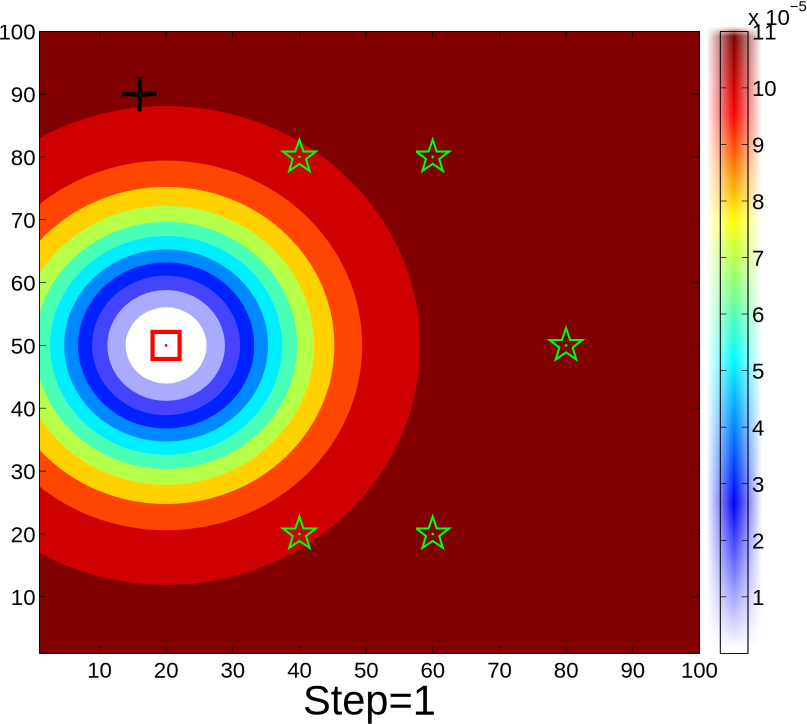
\includegraphics[width=\textwidth]{figures/sta_sen_sta_tar_top2_1_dbf_first}
%			\caption{Individual PDF}\label{fig:sta_sen_sta_tar_top2_init_dbf}
%		\end{subfigure}
%		\begin{subfigure}[b]{0.21\textwidth}
%			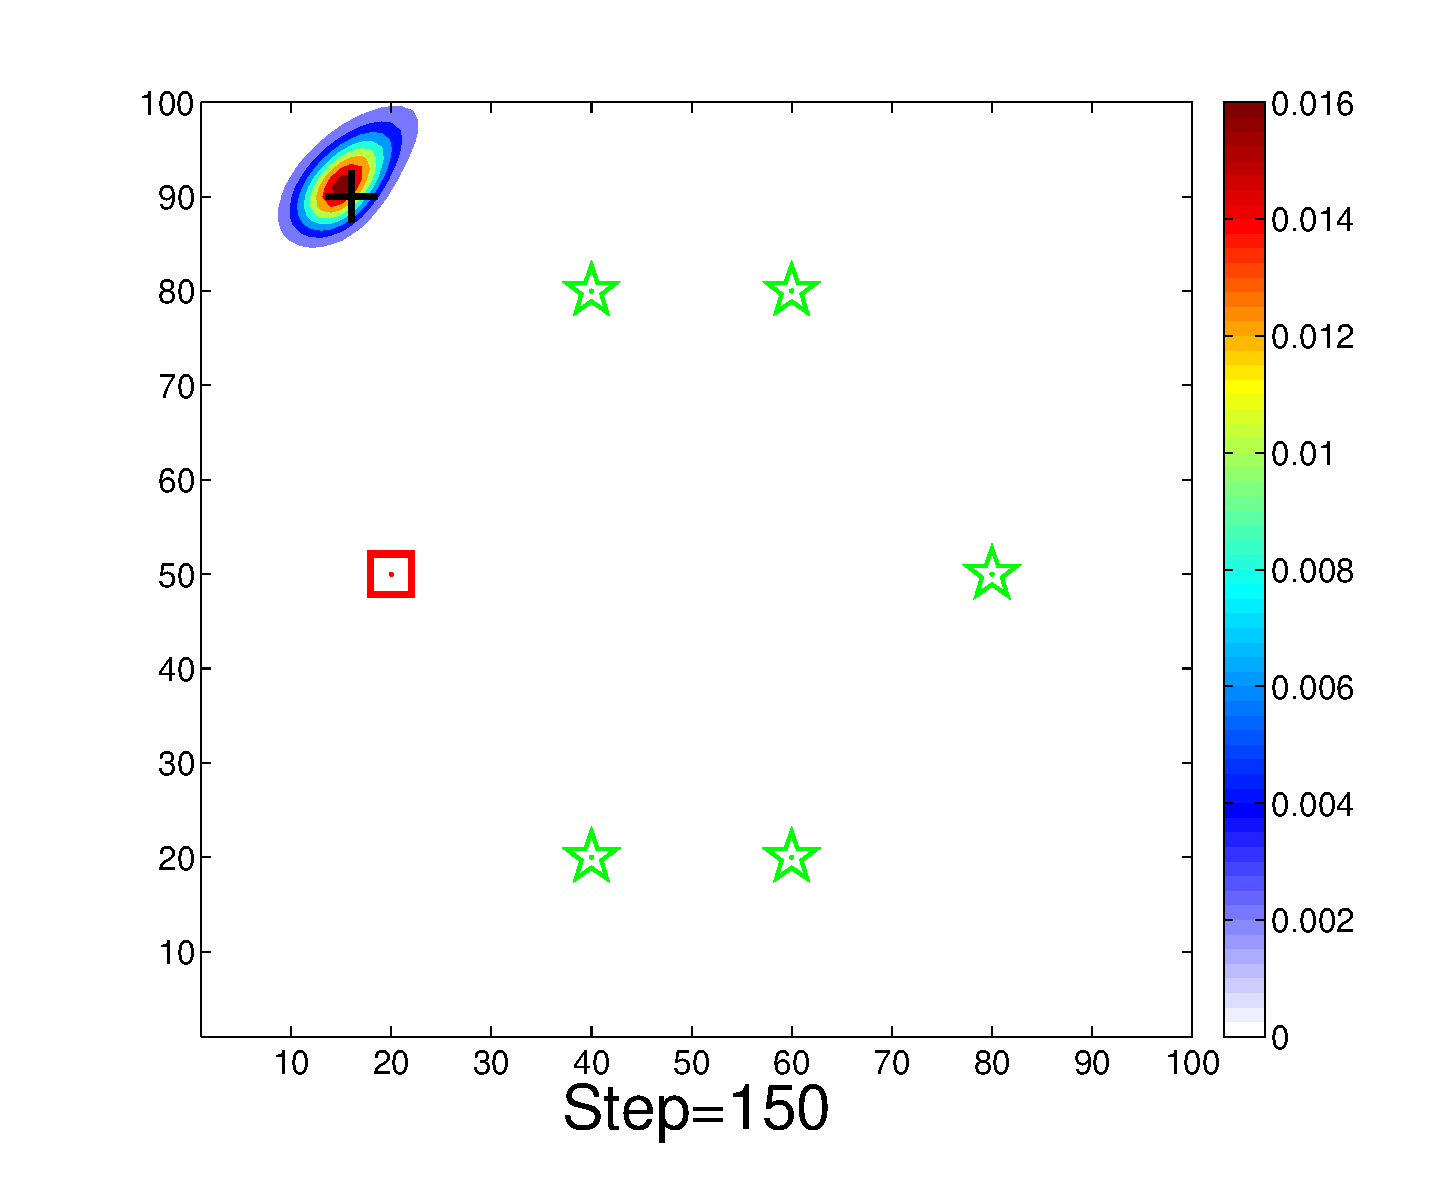
\includegraphics[width=\textwidth]{figures/sta_sen_sta_tar_top2_1_dbf_end}
%			\caption{LIFO-DBF}\label{fig:sta_sen_sta_tar_top2_dbf}
%		\end{subfigure}
%		\begin{subfigure}[b]{0.21\textwidth}
%			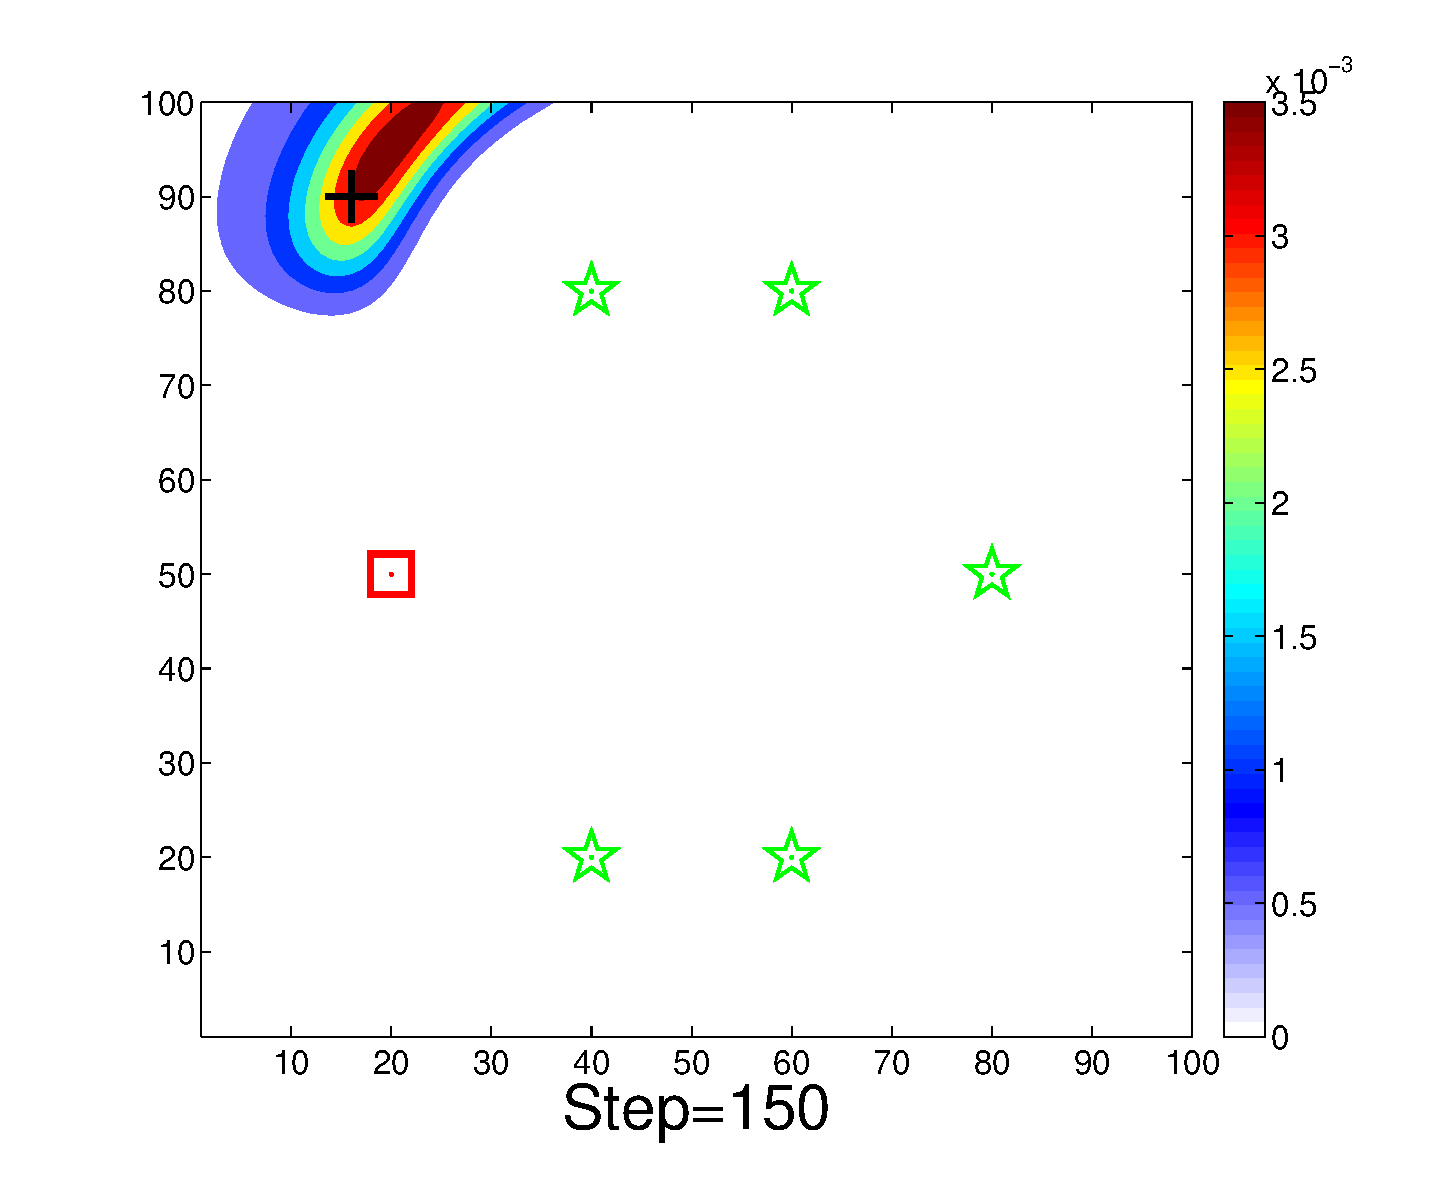
\includegraphics[width=\textwidth]{figures/sta_sen_sta_tar_top2_1_cons_end}
%			\caption{Consensus method}\label{fig:sta_sen_sta_tar_top2_cons}
%		\end{subfigure}
%		\begin{subfigure}[b]{0.21\textwidth}
%			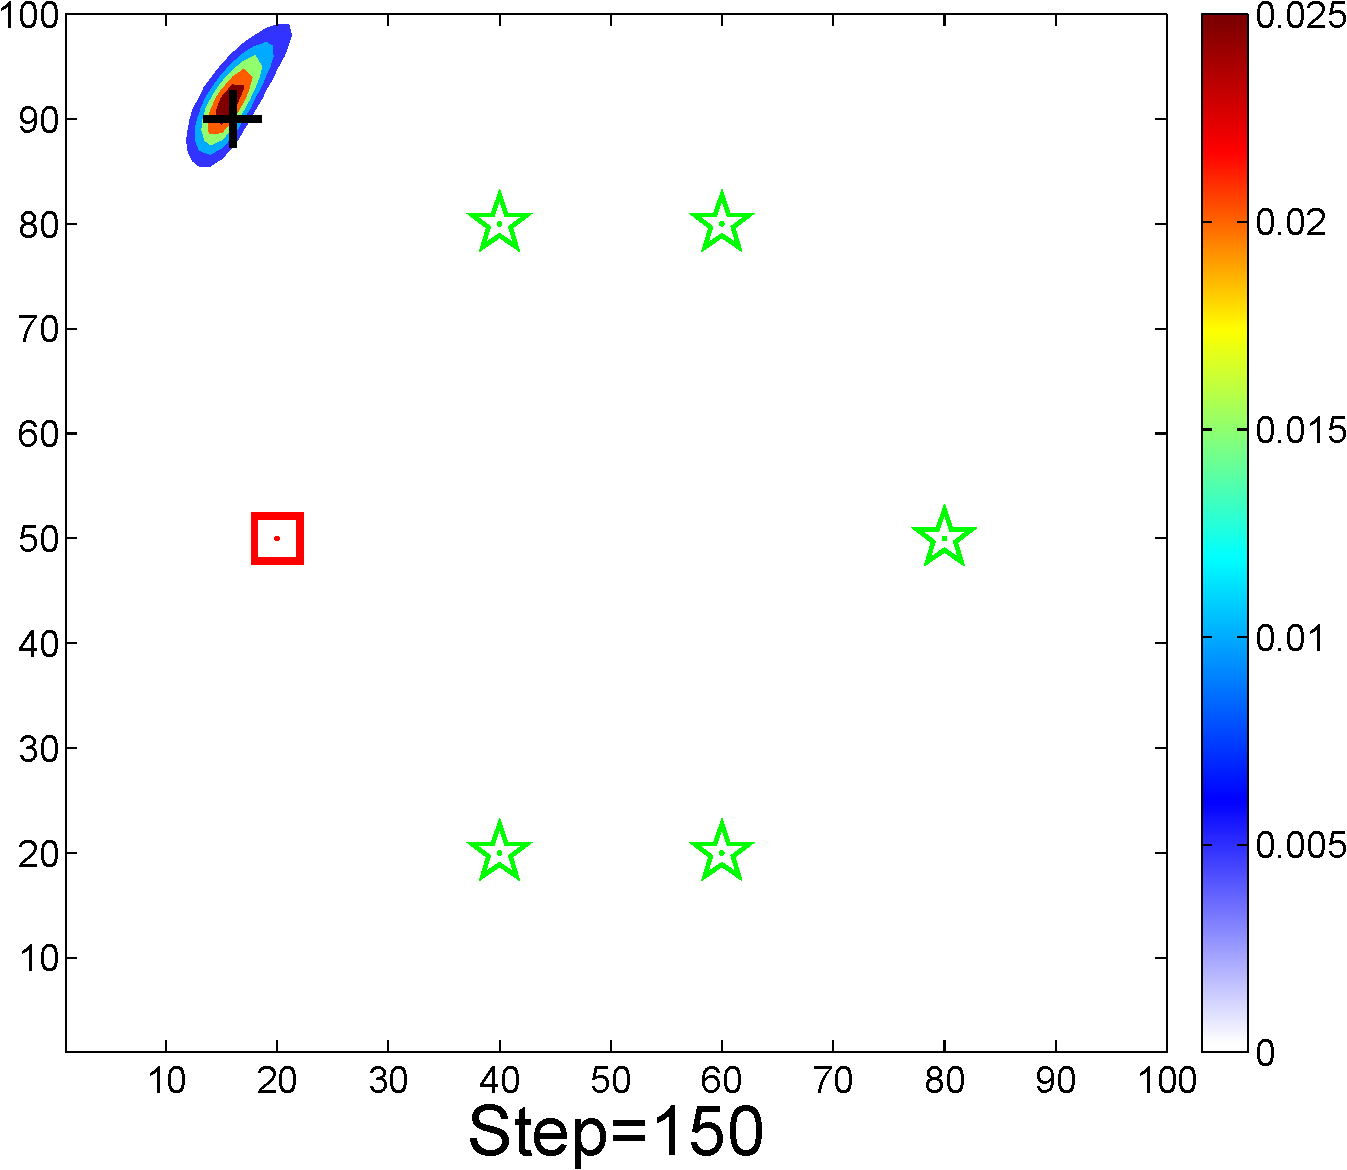
\includegraphics[width=\textwidth]{figures/sta_sen_sta_tar_top2_cent_end}
%			\caption{Centralized filter}\label{fig:sta_sen_sta_tar_top2_cent}
%		\end{subfigure}	
%		\begin{subfigure}[b]{0.23\textwidth}
%			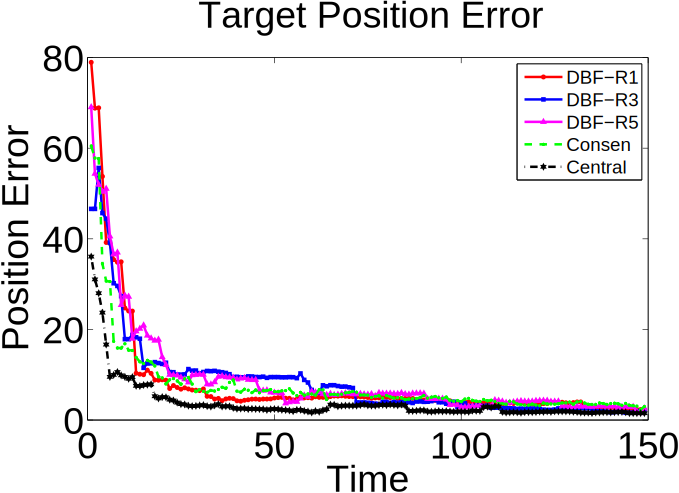
\includegraphics[width=\textwidth]{figures/sta_sen_sta_tar_top2_pos_err}
%			\caption{Position error}\label{fig:sta_sen_sta_tar_top2_pos_err}
%		\end{subfigure}	
%		\begin{subfigure}[b]{0.23\textwidth}
%			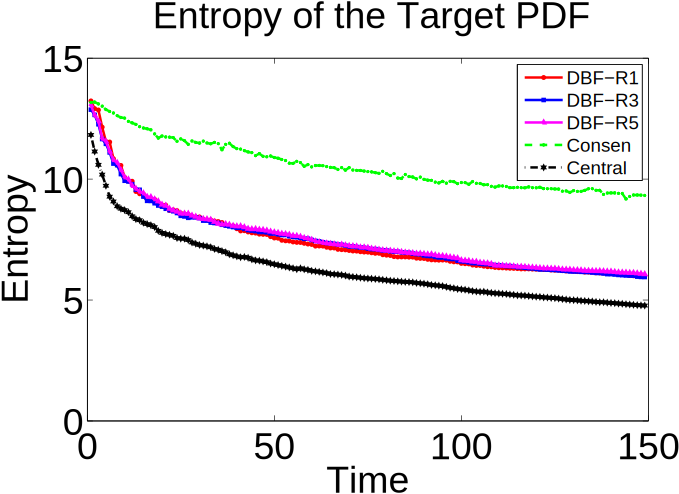
\includegraphics[width=\textwidth]{figures/sta_sen_sta_tar_top2_entropy}
%			\caption{Entropy reduction}\label{fig:sta_sen_sta_tar_top2_entropy}
%		\end{subfigure}		
%		\caption{Second scenario consists of three types of topologies. (b)-(d) show individual PDFs for $1^\text{st}$, $2^\text{nd}$ and $5^\text{th}$ UGV, respectively.}
%			Individual PDFs for three switching interaction topologies: (b)-(e) The $1^\text{st}$ UGV's individual PDFs; (f)-(i) The $2^\text{nd}$ UGV's individual PDFs; (j)-(m) The $5^\text{nd}$ UGV's individual PDFs. }
%		\label{fig:sta_sen_sta_tar2}
%		\vspace{-1.3em}
%	\end{figure}				
		
	This section simulates a set of dynamically changing interaction topologies to demonstrate the effectiveness of LIFO-DBF.
	The scenario includes six static UGVs, represented as the square and stars in \cref{fig:sta_sen_sta_tar1}. % and \cref{fig:sta_sen_sta_tar2}.
	The square represents the UGV whose individual PDF is shown in the figures.
	UGVs are equipped with binary sensors and the sensor model, \cref{eqn:bin_sensor1,eqn:bin_sensor0}, takes the form of Gaussian functions \cite{bonnie2012modelling}:
	%\small\begin{align}\label{eqn:gauss_sensor}
	\small\begin{subequations}\label{eqn:gauss_sensor}
		\begin{align}
			P(z^i_k=1|x^T;x^{R,i})&=e^{-\frac{1}{2}(x^T-x^{R,i})^T{\Sigma}^{-1}(x^T-x^{R,i})},\\
			%		\exp\left\lbrace -\frac{1}{2}(x^T-x^R)^T{\Sigma}^{-1}(x^T-x^R)\right\rbrace \\
			P(z^i_k=0|x^T;x^{R,i})&=1-P(z^i_k=1|x^T;x^{R,i}).
		\end{align}
	\end{subequations}\normalsize
	%\end{align}\normalsize
	%where $x^s$ denotes the UGV position where current observation is obtained. 
	%Figure 4 shows the 1-D illustration of Gaussian binary sensor model.
	%where $x^R$ denotes the UGV position, which is included in UGV state $y^R$.
	
	In the simulation, LIFO-DBF is compared with two commonly adopted approaches in multi-agent filtering: the consensus-based distributed filtering (CbDF) method and the centralized filtering (CF) method.
	The CbDF requires robots to continually exchange their individual PDFs with direct neighbors, using the average of all received and its own individual PDFs as the updated individual PDF.
	Multiple rounds of communication and averaging are conducted at each time step to ensure the convergence of each robot's individual PDF.
	The CF assumes a central unit that can constantly receive and fuse all robots' latest observations into a single PDF.
	10 test trials with randomly generated initial target positions are run and each trial is terminated after 150 time steps.
	The average error between the estimated and true target position and the average entropy of individual PDFs of all 10 trials are compared among these three approaches.
	
%	In the simulation, each UGV forms a circular individual PDF after the initial observation, centered at its own position, as shown in \cref{fig:sta_sen_sta_tar_top1_init_dbf}.
	\cref{fig:com_topo1} illustrates the collection of two topologies for the simulation, the union of which is designed to be jointly connected.
	These two topologies appear alternatively such that their union are connected frequently enough.
	\cref{fig:sta_sen_sta_tar_top1_init_dbf} shows the individual PDF of a UGV after the initial observation.
%	The circular PDF occurs because the Gaussian sensor model (\Cref{eqn:gauss_sensor}) only depends on the distance between a UGV and the target.
	As more observations are received by each UGV, the posterior individual PDF concentrates to the true location of the target (\cref{fig:sta_sen_sta_tar_top1_dbf}), which accords with the consistency of LIFO-DBF.	
	
	Comparison of the estimation performance between LIFO-DBF, CbDF and CF is presented in \cref{fig:sta_sen_sta_tar_top1_pos_err,fig:sta_sen_sta_tar_top1_entropy}.
	Unsurprisingly, the CF achieves the best performance in terms of both small position estimation error and fast reduction of entropy. 
	This happens because the central unit has access to the latest observations of all UGVs, thus making most use of all available information.
	LIFO-DBF and CbDF show similar performance as the CF does in position estimation error.
	However, they significantly differ in terms of entropy reduction. 
	In fact, LIFO-DBF has similar asymptotic performance as the CF in reducing the entropy of PDF over time; this is notable since each UGV only communicates with its neighboring UGVs, which consumes less communication recourse than the CF.
	The CbDF, on the contrary, is much slower in entropy reduction while incurring huge communication burden due to multiple rounds of consensus at each time step.
	The difference in entropy reduction makes sense since CbDF can only ``implicitly" fuses different robots' observation via computing the average of individual PDFs while LIFO-DBF and CF can directly utilize observations, thus making better use of available information.	
	Such difference results in vastly different individual PDFs, as shown in \cref{fig:sta_sen_sta_tar_top1_dbf,fig:sta_sen_sta_tar_top1_cons,fig:sta_sen_sta_tar_top1_cent}, which show the PDF at the end of simulation.
%	Similar performance difference among LIFO-DBF, CbDF and CF for the second scenario can be observed in \cref{fig:sta_sen_sta_tar2}.
	
	\begin{figure}%[thpb]
		\centering
		\begin{subfigure}[b]{0.3\textwidth}
			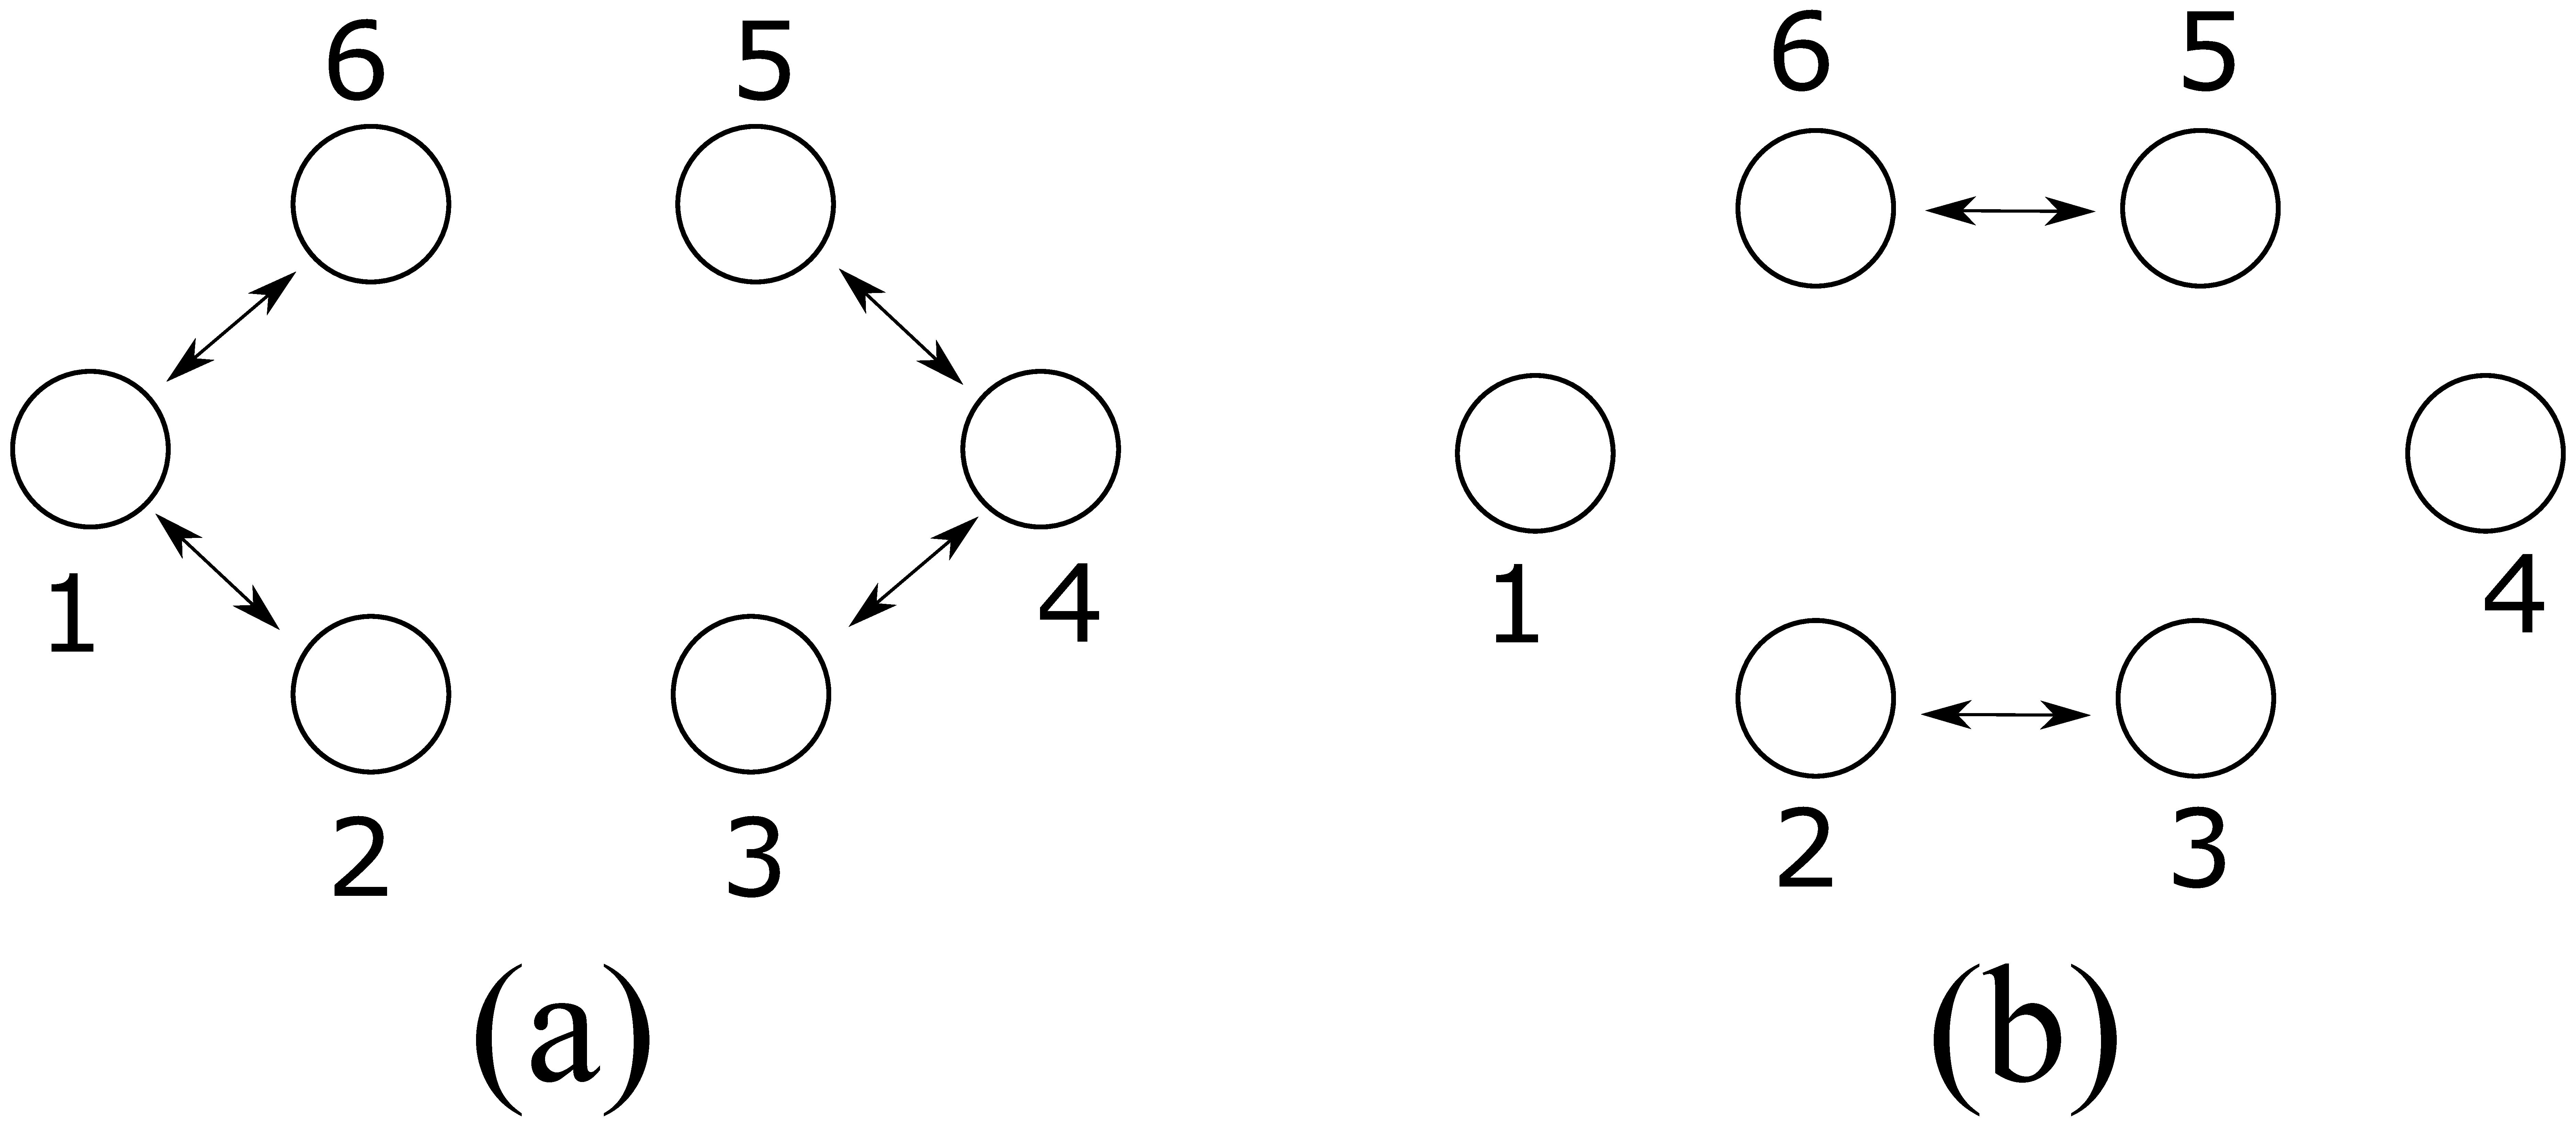
\includegraphics[width=\textwidth]{figures/com_topo1}
			\caption{Collection of changing topologies}\label{fig:com_topo1}
		\end{subfigure}
		~
		\begin{subfigure}[b]{0.2\textwidth}
			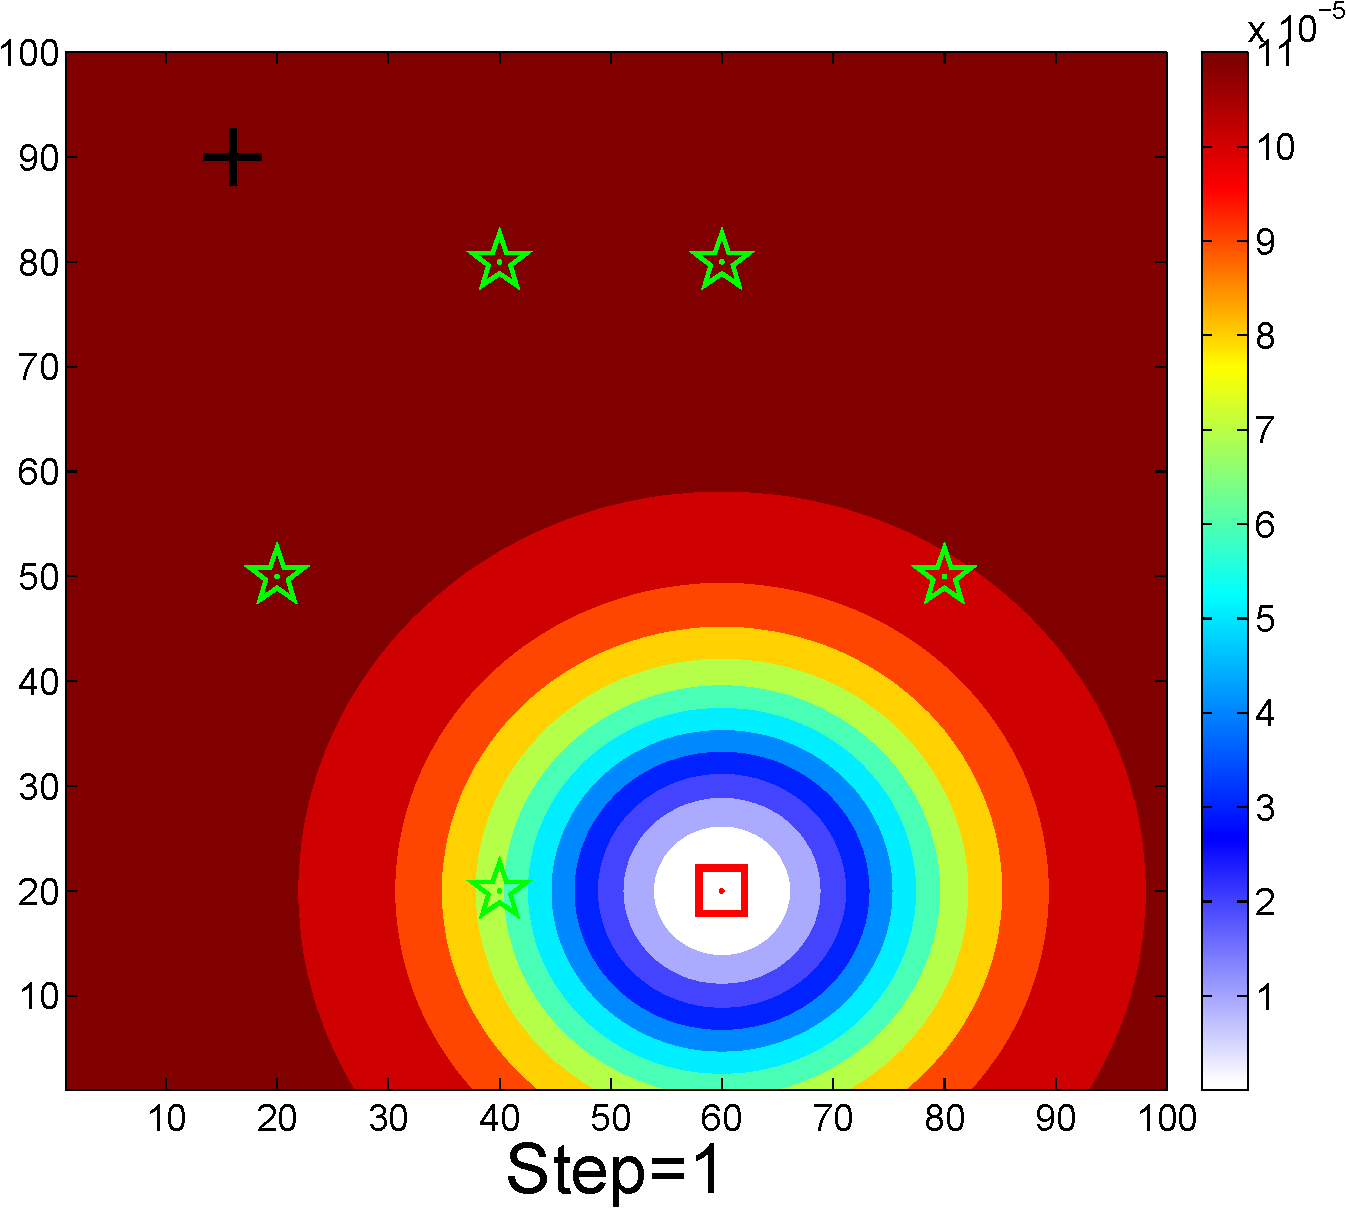
\includegraphics[width=\textwidth]{figures/sta_sen_sta_tar_top1_3_dbf_first}
			\caption{Individual PDF}\label{fig:sta_sen_sta_tar_top1_init_dbf}
		\end{subfigure}
		\begin{subfigure}[b]{0.2\textwidth}
			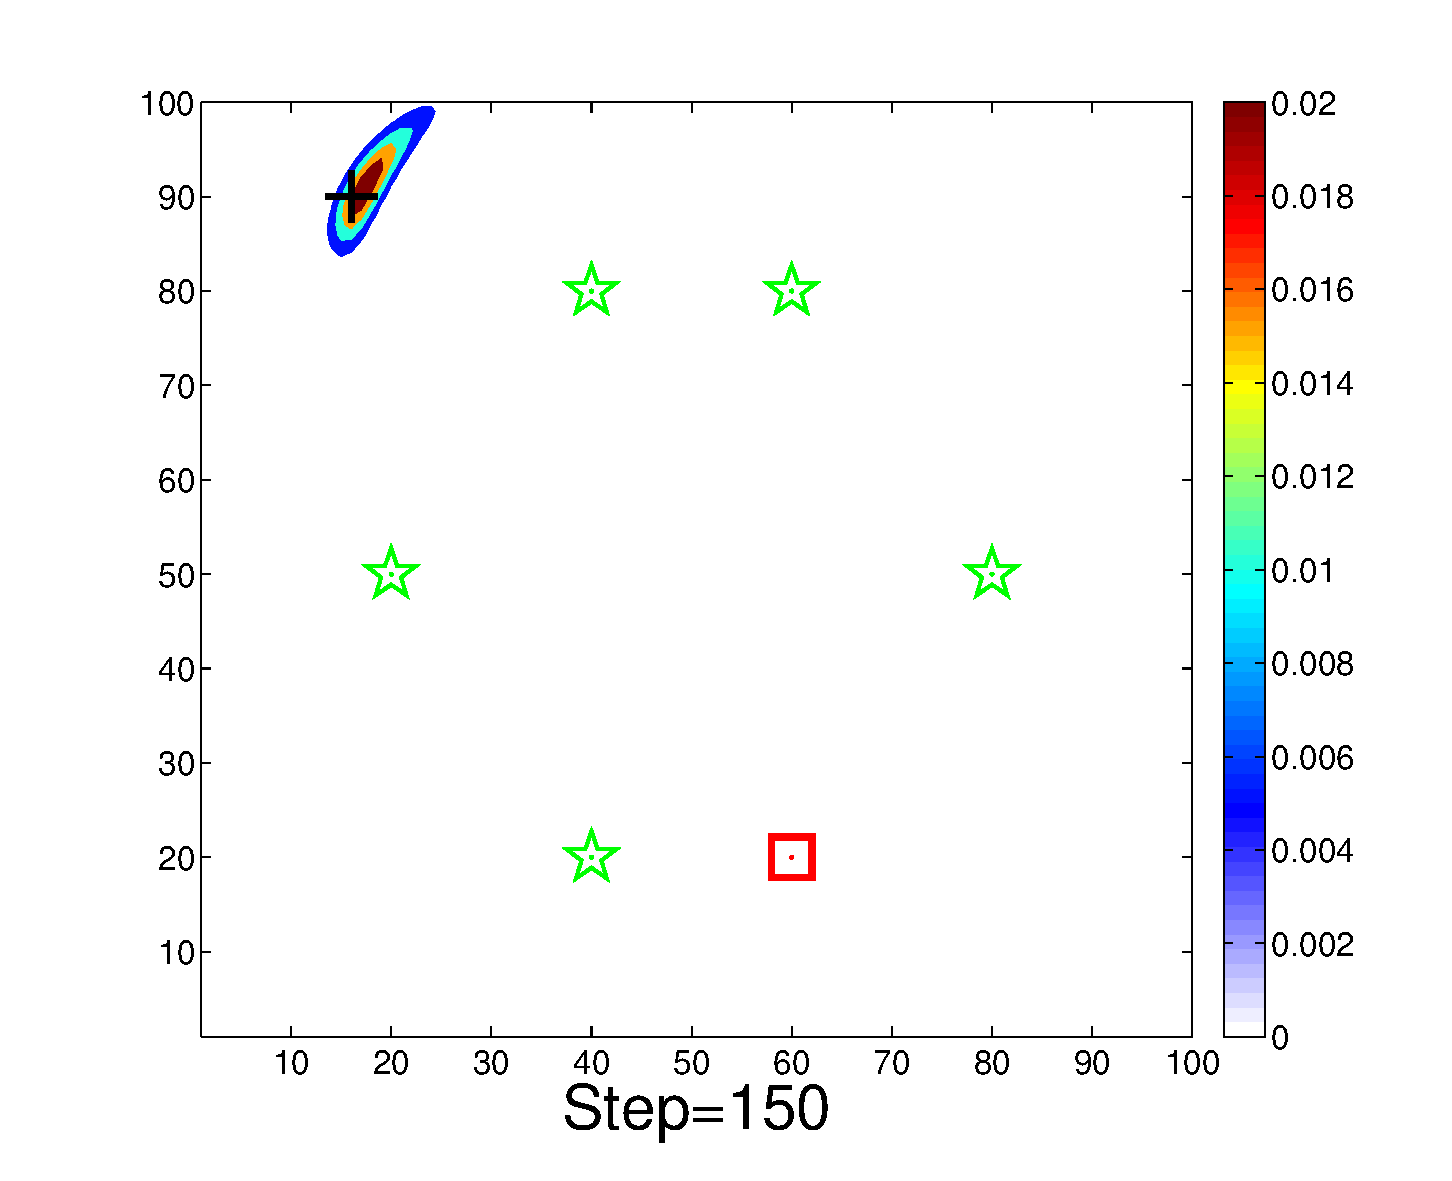
\includegraphics[width=\textwidth]{figures/sta_sen_sta_tar_top1_3_dbf_end}
			\caption{LIFO-DBF}\label{fig:sta_sen_sta_tar_top1_dbf}
		\end{subfigure}
		\begin{subfigure}[b]{0.2\textwidth}
			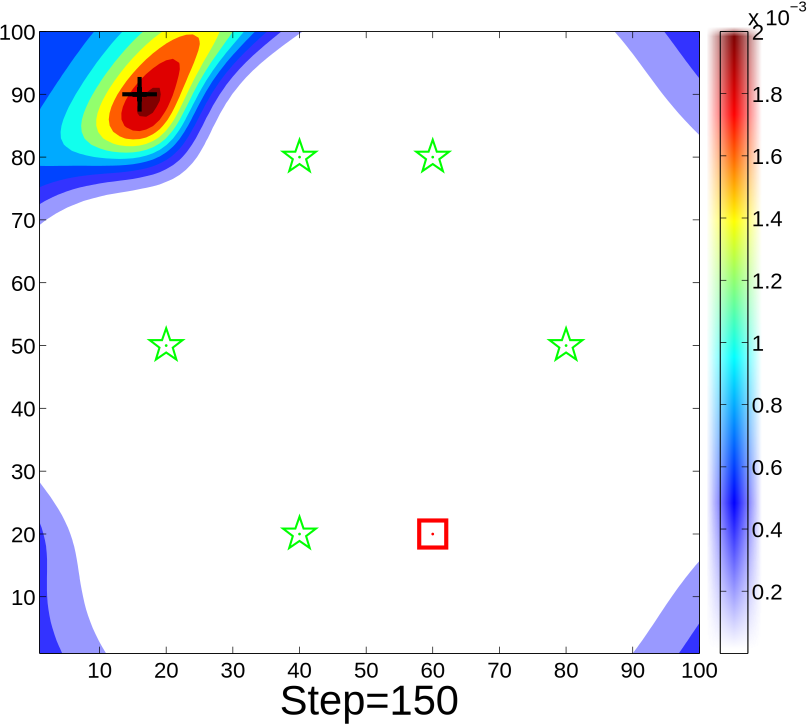
\includegraphics[width=\textwidth]{figures/sta_sen_sta_tar_top1_3_cons_end}
			\caption{Consensus method}\label{fig:sta_sen_sta_tar_top1_cons}
		\end{subfigure}
		\begin{subfigure}[b]{0.2\textwidth}
			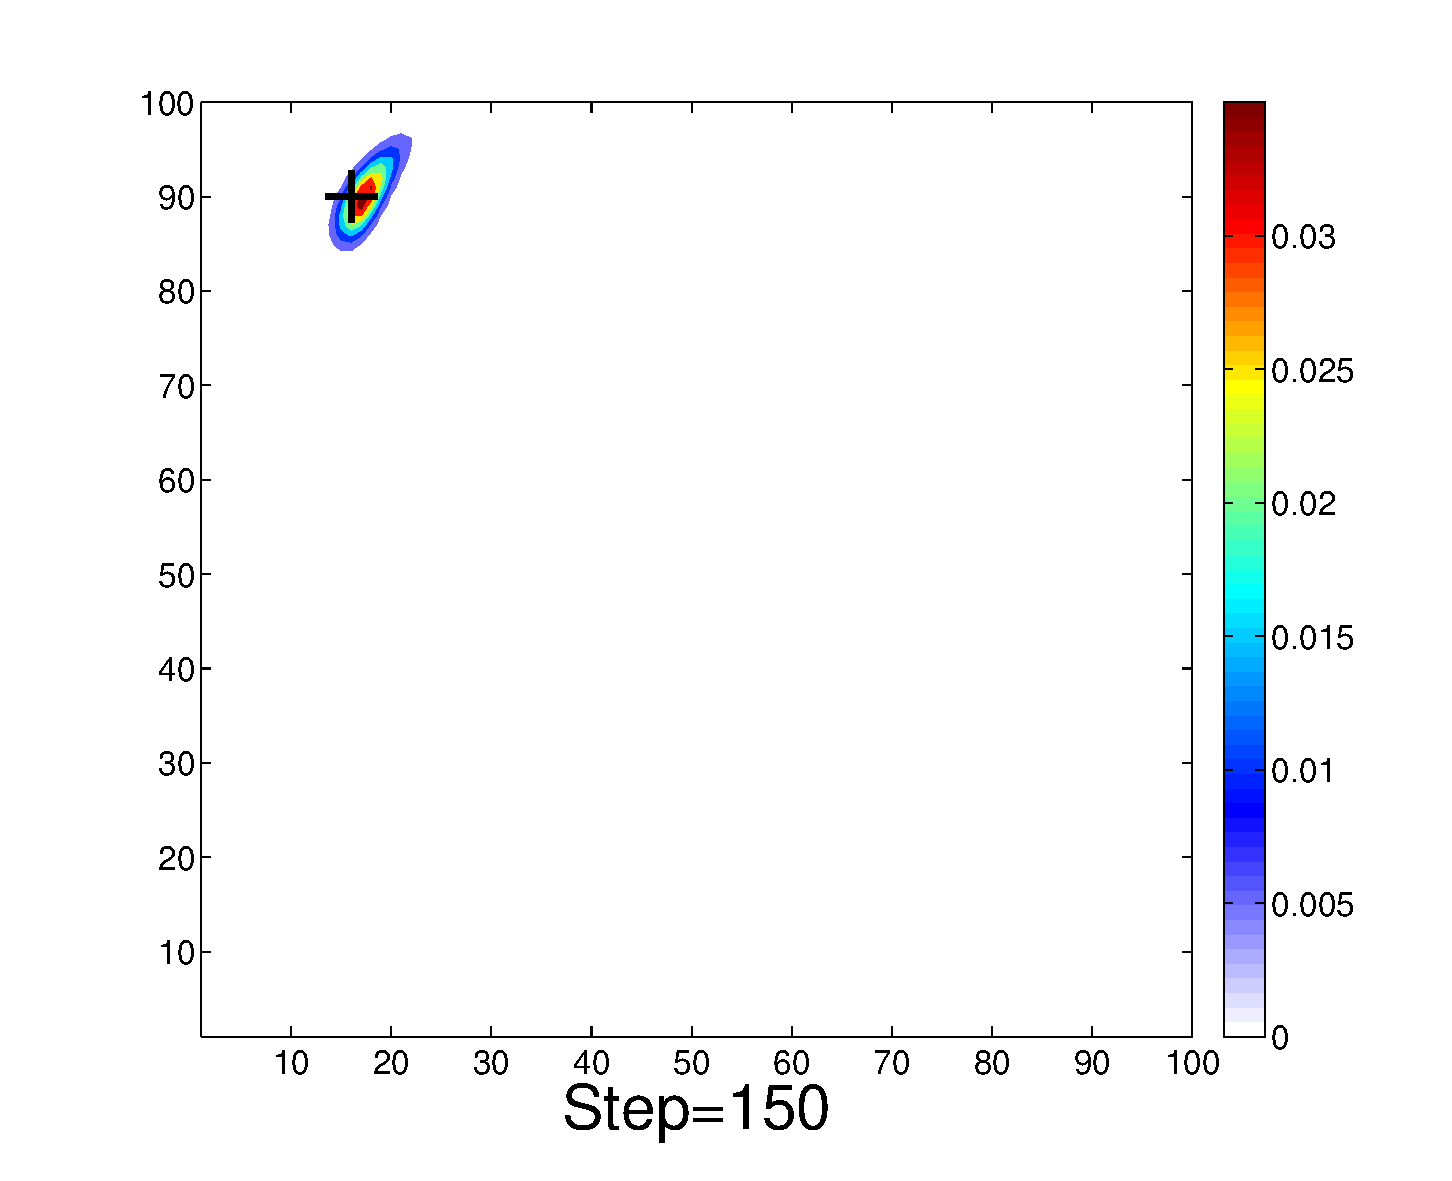
\includegraphics[width=\textwidth]{figures/sta_sen_sta_tar_top1_cent_end}
			\caption{Centralized filter}\label{fig:sta_sen_sta_tar_top1_cent}
		\end{subfigure}	
		\begin{subfigure}[b]{0.21\textwidth}
			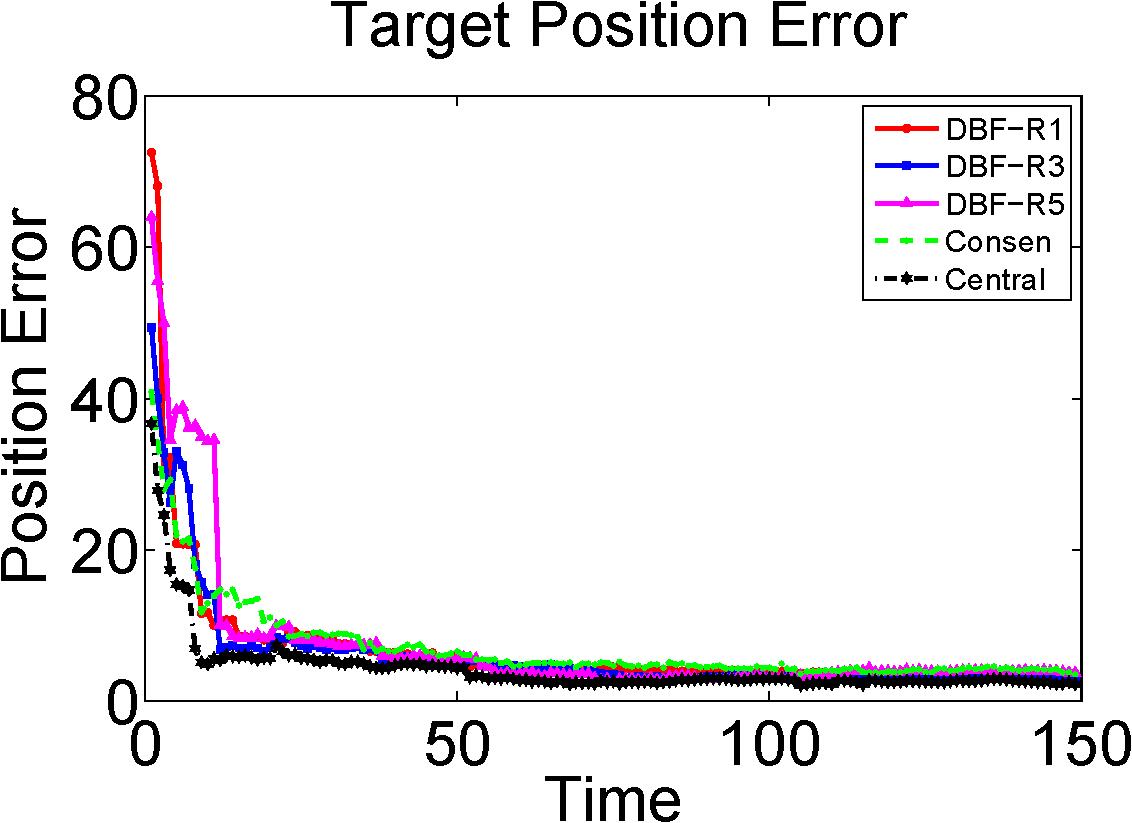
\includegraphics[width=\textwidth]{figures/sta_sen_sta_tar_top1_pos_err}
			\caption{Position error}\label{fig:sta_sen_sta_tar_top1_pos_err}
		\end{subfigure}	
		\begin{subfigure}[b]{0.21\textwidth}
			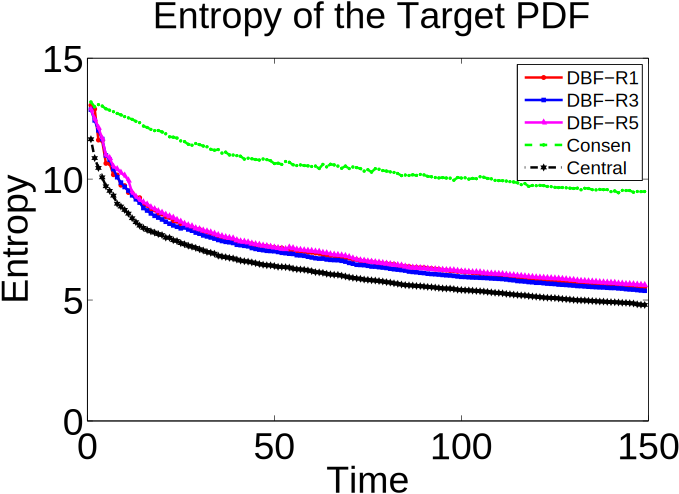
\includegraphics[width=\textwidth]{figures/sta_sen_sta_tar_top1_entropy}
			\caption{Entropy of PDF}\label{fig:sta_sen_sta_tar_top1_entropy}
		\end{subfigure}		
		\caption{(a) two interaction topologies; (b) individual PDF of the $3^\text{rd}$ UGV after initial observation; (c)-(e) PDFs at the end of simulation using different filters; (f) average position estimation errors; (g) average entropy. In last two figures, individual PDFs of the $1^\text{st}$, $3^\text{rd}$ and $5^\text{th}$ UGV using LIFO-DBF, the common PDF using CbDF and using CF are compared.}
		\label{fig:sta_sen_sta_tar1}
		\vspace{-1.5em}
	\end{figure}
	
	
	\section{CONCLUSION}\label{sec:conclu}	
	This paper presents a measurement dissemination-based distributed Bayesian filtering (DBF) method for a network of multiple unmanned ground vehicles (UGVs) under dynamically changing interaction topologies.
	The information exchange among UGVs relies on the Latest-In-and-Full-Out (LIFO) protocol, which significantly reduces the transmission burden between each pair of UGVs to scale linearly with the network size.
	Under the condition that the union of undirected switching topologies is connected frequently enough,
	LIFO can disseminate observations over the network within finite time. 
%	The LIFO-based DBF algorithm is then derived to estimate individual probability density function for target localization in a static environment. 
%	The consistency of this algorithm is proved by utilizing the law of large numbers, ensuring that each individual estimate of target position converges in probability to the true value.
	The consistency of LIFO-DBF is proved, ensuring that each individual estimate of target position converges in probability to the true value.
%	Simulations comparing LIFO-DBF with consensus-based distributed filters (CbDF) and the centralized filter (CF) show that LIFO-DBF achieves similar performance as CF and superior performance over CbDF while requiring less communication resource.
	Simulations show that LIFO-DBF achieves similar performance as the centralized filter and superior performance over consensus-based distributed filters.
		
	Future work includes handling other types of sensors and directed interaction topologies.
	Other types of sensors may have biased observations and subject to non-Bernoulli distribution, which complicates the design and analysis of LIFO-based Bayesian filters.
	The directed interaction topologies, due to the constraint of unidirectional communication, may affect condition for the consistency of LIFO-DBF. 
	
	
	\addtolength{\textheight}{-12cm}   % This command serves to balance the column lengths
	% on the last page of the document manually. It shortens
	% the textheight of the last page by a suitable amount.
	% This command does not take effect until the next page
	% so it should come on the page before the last. Make
	% sure that you do not shorten the textheight too much.
	
	%%%%%%%%%%%%%%%%%%%%%%%%%%%%%%%%%%%%%%%%%%%%%%%%%%%%%%%%%%%%%%%%%%%%%%%%%%%%%%%%
	
	
	
	%%%%%%%%%%%%%%%%%%%%%%%%%%%%%%%%%%%%%%%%%%%%%%%%%%%%%%%%%%%%%%%%%%%%%%%%%%%%%%%%
	
	
	
	%%%%%%%%%%%%%%%%%%%%%%%%%%%%%%%%%%%%%%%%%%%%%%%%%%%%%%%%%%%%%%%%%%%%%%%%%%%%%%%%
	%\section*{APPENDIX}
	%
	%Appendixes should appear before the acknowledgment.
	
%	\section*{ACKNOWLEDGMENT}
%	%This work is supported by the Embedded Humans: Provably Correct Decision Making for Networks of Humans and Unmanned Systems project, a MURI project funded by the Office of Naval Research.
%	The authors gratefully acknowledges the Office of Naval Research for supporting this work. 
%	They would also like to thank Yuting Wei in the Department of Statistics, UC Berkeley for her sincere help and fruitful discussion.
	
	%The preferred spelling of the word �acknowledgment?in America is without an �e?after the �g? Avoid the stilted expression, �One of us (R. B. G.) thanks . . .? Instead, try �R. B. G. thanks? Put sponsor acknowledgments in the unnumbered footnote on the first page.
	
	
	
	%%%%%%%%%%%%%%%%%%%%%%%%%%%%%%%%%%%%%%%%%%%%%%%%%%%%%%%%%%%%%%%%%%%%%%%%%%%%%%%%
	{\footnotesize\bibliographystyle{IEEEtran}}
	%\bibliographystyle{bibtex}
	\bibliography{references}
	
\end{document}
